\chapter{The Standard Model of Particle Physics}
\label{ch:SM}
\begin{flushright}
\textit{\\A physicist is an atom's way of knowing about atoms $\sim$ George Wald\\}
\end{flushright}

\noindent The aim of this chapter is to give a summary of the framework that is used in particle physics.
This framework was developed in stages throughout the latter half of the 20th century and is known as the Standard Model of particle physics.
This model is a quantum field theory that is able to describe most of what is seen in particle physics experiments, and proved to be successful in predicting later experimental discoveries.
In this chapter, a brief historical overview of the development of this theory will be given together with a limited description in order to familiarize the reader with concepts that will be used throughout this work.
For a more in-depth and exhaustive discussion I refer to Refs. \cite{Povh,Peskin:1995ev,Agashe:2014kda,Bettini:2008zz}. We start with an overview of the constituent particles of the Standard Model, linking them to our everyday life. Secondly, a general description is given of the nature of forces. Thirdly, we go to a more mathematical and in-depth description of the Standard Model. Lastly, we present the many successes of this model and finish with an argumentation of why there is a need for physics beyond this model.

\section{What we call matter: fermions}
\label{sec:fermions}
Physics (from Ancient Greek: \gr φυσική \en - $physik\acute{\bar{e}}$, ``knowledge of nature'') is the natural science that studies matter.
Matter is made up of \textit{atoms} (from Greek: \gr ἄτομος \en - \textit{atomos}\footnote{Coined by ancient Greek philosophers Leucippus and his pupil Democritus who believed matter was made up of discrete units.}, ``indivisible'') that can bind together into molecules and account for what is around us in our everyday life.
Atoms are made up of a positively charged \textit{nucleus} that is surrounded by one or more \textit{electrons}. The nucleus and electrons are bound to each other via the electromagnetic force.
The nucleus is made up of one or more \textit{protons} and, typically, an approximately equal amount of \textit{neutrons}. Because of their similar characteristics, protons and neutrons are often referred to as \textit{nucleons} and together they make up more than 99.9\% of an atom's mass.
Nucleons are made up of smaller particles called \textit{quarks}\footnote{The word ``quark'' originally appeared in the novel \textit{Finnegans Wake} written by the Irish author James Joyce (1882–1941). The protagonist of the book dreams that he is serving beer to a drunken seagull. Instead of asking for ``three quarts for Mister Mark'' the inebriated bird says ``three quarks for Muster Mark''. Murray Gell-Man had the habbit of using names like ``squeak'' and ``squork'' for peculiar objects and after encountering the sentence in the book the name struck him as appropriate since the (then hypothetical) particle came in threes.}, which are, as far as we know, \textit{fundamental particles}. This means that we believe that there are no smaller substructures making up these objects and they are in essence mathematically best described as infinitely small.
Because of this, they are often referred to as pointlike.
In the Standard Model (SM), these particles are found to be \textit{fermions}, which have odd half-integer spins, obeying the laws of quantum mechanics.
The spin of a particle is often illustrated with its classical counterpart in which an object is spinning and thus carries an intrinsic angular momentum.
This analogy cannot be extrapolated to pointlike particles, but the property happens to hold the same units as the classical orbital momentum.
The spin of a particle seems to be just another property particles have, like charge or mass.
Fermions follow Fermi-Dirac statistics and therefore obey the Pauli exclusion principle. As a consequence, fermions cannot occupy the same place at the same time (more formally: no two fermions may be described by the same quantum numbers). This agrees with our macroscopic obeservations of matter in everyday life: matter interacts with matter; people cannot walk through walls!

In total, the SM distinguishes 24 different fermions that can be subdivided into two distinct classes: \textit{quarks} and \textit{leptons}. There are six quarks (up, down, charm, strange, top and bottom), and six leptons (electron, electron neutrino, muon, muon neutrino, tau and tau neutrino), along with the corresponding antiparticle for each of these fermions.
A summary of all the particles in the Standard Model is given in Figure \ref{SMparticles}.

\begin{figure}[t]
\centering
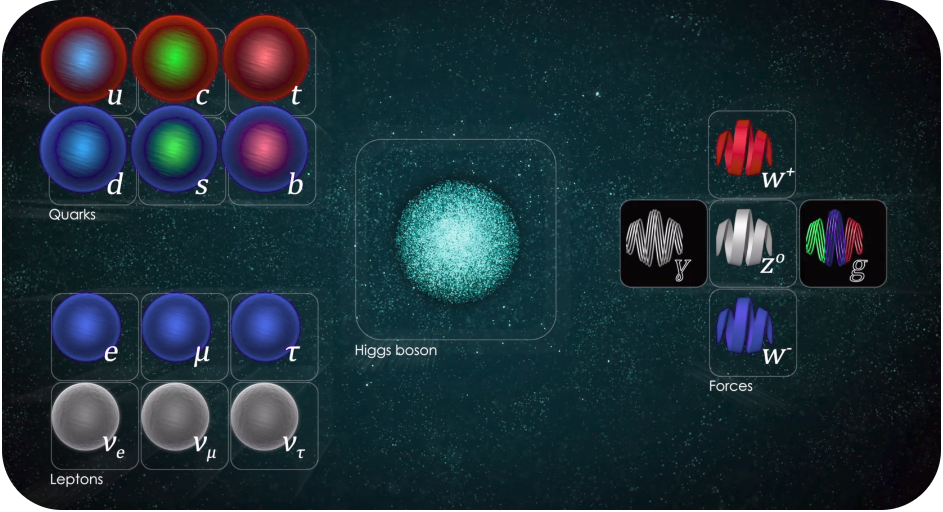
\includegraphics[width = \textwidth]{chapter1/img/SMparticles_rounded}
\caption{The Standard Model of particle physics distinguishes fermions (left) from bosons (right). The Brout-Englert-Higgs boson (middle) is more peculiar as it has no intrinsic spin and plays a special role in the theory. Charges for fermions are not explicitly written to account for antiparticles. Illustration from Ref. \cite{cernSMpic}.}
\label{SMparticles}
\end{figure}

\subsection{Leptons}
Leptons\footnote{\gr λεπτός \en (leptos) meaning thin, delicate, lightweight, or small. Originally, leptons were considered the ``light'' particles and hadrons the ``heavy'' particles, but the discovery of the tau lepton in 1975 broke that rule.} can be subdivided in two classes: electromagnetically charged particles ($e^-$, $\mu^-$ and $\tau^-$) and the neutral neutrinos\footnote{The Italian word for neutron (neutrone) sounds like the word neutral (neutro) with an augmentative suffix (-one) tacked on the end, making the word a little wordplay. In Italian, it sounds something like ``big neutral''. Replace the augmentative suffix -one with the diminutive suffix -ino and you have a ``little neutral'', which is a good description of what a neutrino is — a diminutive neutral particle.} ($\nu_{e}$, $\nu_{\mu}$ and $\nu_{\tau}$). Because of their charge, electrons are the well-known particles that combine together with nucleons into atoms. Being the lightest of the three charged leptons, the electron is said to be part of the first \textit{generation}, together with the electron neutrino. Muons differ only from electrons in mass\footnote{This characteristic is often referred to as \textit{lepton universality.}} and make up the second generation together with muon neutrinos. Similarly, tau particles and tau neutrinos define the third generation. All leptons have a corresponding antiparticle indicated by a positive charge (e.g. $e^+$) or a bar (e.g. $\bar{\nu}_e$). Neutrinos are proven to have a very small mass \cite{RevModPhys.88.030502} and interact only via the weak force (Section \ref{subsec:weak}), making them inherently very hard to detect.

\subsection{Quarks}
\label{sub:quarks}
The six quarks are called up, down, charm, strange, top and bottom quarks $((u,d),(c,s),(t,b))$.
Each generation is made up of a particle with charge +2/3 and one with -1/3 (also visualized in Figure \ref{SMparticles}). These charges are multiples of the absolute electron charge.
The difference between generations is again essentially the bare mass of the particles. Because quarks also interact through the strong force (see Section \ref{subsec:strong}), they combine into 
\textit{hadrons\footnote{\gr αδρός \en (adros) meaning thick, robust, massive, or large. This name alludes to the ability of the point-like quarks to bind together and form particles that are massive in a certain sense.}} (of which nucleons are the best known examples). Due to their color charge and the intrinsic behavior of the strong force, quarks cannot be observed freely: they always combine into color neutral particles, a property called \textit{confinement}. When a hadron, with its constituent quarks, is pulled apart, the attractive force between the quarks does not fall down rapidly since gluons carry color charge themselves. When these particles are pulled apart far enough, it becomes energetically more favorable to produce new quark-antiquark pairs, which again combine into color neutral particles\footnote{This process is called \textit{hadronization} and results into the production of ``jets'' in particle accelerators \cite{cmsjetsurl}.}. The energy requirement for the production of new particles is far below the one to separate the quarks far enough from each other to observe them separately. Antiquarks are again denoted with a bar (i.e. $\bar{u}$).

Because of their ability to interact via the strong force, particle accelerators in the 1960s led to the discovery of a plethora of possible quark combinations, something that is often referred to as the ``particle zoo''.



\section{How particles communicate: interactions}

There are four fundamental interactions known to exist: \underline{gravity} and \underline{electromagnetism}, which produce significant long-range forces, and the \underline{strong} and \underline{weak forces} that only express themselves at (sub)atomic distances and govern nuclear interactions. These are explained in more detail below and an overview is given in Table \ref{tab:forces}.

Particles interact with each other through the exchange of \textit{gauge bosons} or \textit{force carriers}\footnote{A classic and very simplistic way of looking at force carriers is to imagine two people standing on a boat. The force carrier is a heavy ball that can be thrown from one person to the other. Doing so, both persons will move in opposite direction.}. Gauge bosons are bundles of energy, \textit{quanta}, and can be seen as excitations of one of the force fields.

Fields are a mathematical approach used by physicists to describe what we observe in experiments. Although the use of fields is very natural, the concept might feel a bit unfamiliar. In the following, the known forces are described in more detail. Gravity plays less of a role in subatomic physics, but is added for completeness and is mainly used to make the reader more familiar with the concept of a field.

\begin{table}[]
\centering
%\begin{footnotesize}
\caption{Summary of the known forces and their properties. The relative strengths are quoted in terms of a dimensionless coupling constant ($\alpha_g, \alpha_w, \alpha$ and $\alpha_s$). These ``constants'' actually depend on the energy. These number were obtained from Ref. \cite{hyperphysicsStrengths}.}
%Ref: https://web.archive.org/web/20160304133522/https://www.pha.jhu.edu/~dfehling/particle.gif. A nice webpage explaining... :https://profmattstrassler.com/articles-and-posts/particle-physics-basics/the-known-forces-of-nature/the-strength-of-the-known-forces/
%http://web.mit.edu/sahughes/www/8.022/lec01.pdf}
\label{tab:forces}
\resizebox{\textwidth}{!}{%
\begin{tabular}{|l |c|c|c|c|}
\hline
\cellcolor[HTML]{F1A91E} & \cellcolor[HTML]{F1A91E}                              & \cellcolor[HTML]{F1A91E}\textbf{Weak} & \cellcolor[HTML]{F1A91E}\textbf{Electromagnetic} & \cellcolor[HTML]{F1A91E}\\ 
\multirow{-2}{*}{\cellcolor[HTML]{F1A91E}\textbf{Interaction}} & \multirow{-2}{*}{\cellcolor[HTML]{F1A91E}\textbf{Gravitational}} & \multicolumn{2}{c|}{\cellcolor[HTML]{F1A91E}\textbf{Electroweak}}               &      \multirow{-2}{*}{\cellcolor[HTML]{F1A91E}\textbf{Strong}}                \\ \hline
\textbf{Acts on} &mass/energy  & weak flavor  & electric charge & color charge  \\ \hline
\textbf{Couples to}  & all particles & all fermions   & electrically charged particles & quarks, gluons \\ \hline
\textbf{Mediation}                                 & not yet observed                                      & $W^+, W^-,Z$                 & $\gamma$                                & gluons \\ \hline
\textbf{Rel. strength} & $10^{-39}$ & $10^{-6}$ & 1/137 & 1 \\ \hline
%Long-distance                              & $\frac{1}{r^2}$                                        & $\frac{1}{r}e^{-m_{W,Z}\cdot r}$   & $\frac{1}{r^2}$                          & \multicolumn{2}{c|}{$r$} \\ \hline
\end{tabular}%
}
%\end{footnotesize}
\end{table}

\subsection{Gravity}
Gravity (from Latin/old French: gravitas/grave, ``weighty, heavy'') is the phenomenon wherein massive objects are attracted to each other. Gravitation is famously described by the theory of general relativity proposed by Einstein in 1915. Compared to the other forces, gravity is intrinsically very weak\footnote{Two magnets that fit in the palm of your hand can deliver a force which is of similar strength as the force that our entire planet exerts on a human body.} and is not described in the SM (see Section \ref{sec:sm}). This is why gravity is often left out in discussions of particle physics experiments, but is crucial for understanding astronomical objects and how they influence each other. It can, however, be used to explain the concept of a field in a very natural way.

A very good description of gravitation was already provided centuries ago. First published on July 5th, 1686 was Newton's work \textit{Philosophiae Naturalis Principia Mathematica} (``the Principia'') that first introduced several formulas that are still widely used today. The equation of the force exerted by two massive bodies takes the following form,
\begin{equation}
F = G \frac{m_1 m_2}{r^2},
\end{equation}
where $F$ is the gravitational force acting between two objects, $m_1$ and $m_2$ are the masses of the objects, $r$ is the distance between their center of mass, and $G$ is the gravitational constant.

Newton's law states that two massive bodies will exert a force on one another that is proportional to their masses, but inversely proportional to the square of the distance between them. Newton realized this would mean that at any given instant in time all massive objects in the universe would know from every other object in the universe where it is located and how massive it is\footnote{Imagine the attraction of the Moon to the Earth: how are both ``communicating''?}. Because of this, Newton himself believed his explanation could not be the final answer. The answer is fully described in Einstein's work of general relativity, but the first idea in the right direction was introduced by Laplace in 1783. Laplace explained that massive objects do not ``feel'' each other but distort space and time in such a way that objects that are attracted, ``fall'' towards each other. Field theory makes it possible to treat the laws of physics as a local property instead of an action from a distance.


To date, it has not been possible to describe gravity in the framework of quantum field theory like the other fundamental forces, although, there is still much ongoing work. The gauge bosons from such a quantum field theory for gravity are mostly referred to as \textit{gravitons}.

\subsection{Electromagnetism}
The electromagnetic field (from Ancient Greek: \gr ἤλεκτρον \en $\bar{e}lektron$, ``amber'', and \gr μαγνῆτις λίθος, \en \textit{magnetis lithos}, which means ``Magnesian stone''\footnote{In 1641, Kircher described the magnetic properties of the Magnesian stone in his book \textit{Magne sive de arte magnetica opus tripartitum} \cite{kircher1641athanasii}.}) presents itself in the electrical and magnetical forces. In the late 1870s, the publication of Maxwell's \textit{A Treatise on Electricity and Magnetism} showed that the electric and magnetic interactions of negative and positive charges are mediated by one force: electromagnetism. Particles carrying a charge of one of these forces can attract or repel each other.

Similar to the gravitational field, the electromagnetic field pervades all around us, providing the necessary description of how charged particles interact with each other. The interaction of nuclei, which have a positive electric charge, and electrons makes up most of what is described in chemistry. 

The force carrier of electromagnetism is called a \textit{photon}, or in other words: light.
\subsection{Weak force}
\label{subsec:weak}
The weak force is one aspect of the overarching electroweak theory that combines electromagnetism and the weak force. As opposed to gravity and electromagnetism, it only takes place at very small subatomic distances\footnote{The reason being is that the force carriers are massive; more info in Section \ref{sec:sm}.}. One well known phenomenon that is governed by the weak force is \textit{beta decay} in which free neutrons decay into protons and produce an extra electron and antielectron neutrino. Another beautiful example of the weak force is the driving mechanism in the Sun's thermonuclear process that makes it shine. This process cannot be explained by chemical processes but with the fusion of hydrogen cores into helium where two out of four protons are converted to neutrons. This conversion of the proton into a neutron is explained by the weak force.

The force carriers of the weak force are the $W^+$, $W^-$ and $Z$ bosons. 
Quantum field theory tells us that the interaction strength of particles depends on the coupling constants and the properties of the mediator particles. The coupling constants of the weak force are of similar magnitude as those in electromagnetism. However, because of the mass of the weak force carriers, the interaction strength at low energies, such as radioactive decay, becomes much smaller\footnote{The mediator term for photons scales with $\frac{1}{q^2}$ with  $q$ the momentum of the mediator. $W$ and $Z$ boson mediator terms scale with $\frac{1}{q^2 - M^2}$ with $M$ the mass of the mediator. When $q$ is low, for example in radioactive decays, this term becomes very small due to the mass of the bosons. On the other hand, if $q$ and $M$ are of similar magnitude, the weak force is strong. For example, the top quark decay will most likely happen via the weak force.}. This makes the force seem weak, hence the name\footnote{It was Fermi who first came up with a proper description of the beta decay in 1933. However, he described the interaction as a 4-point interaction, making it only valid up to energies below 100 GeV.}.\\

\noindent The weak force also has some peculiar properties that are unique in a number of respects:

\vspace{2mm}
\begin{itemize}
\item it is the only interaction that violates parity symmetry and even does so maximally (V-A interaction),
\item its force carriers are massive as opposed to all other force carriers,
\item it is the only force capable of changing quarks from one family into a quark of another family.
\end{itemize}

\subsection{Strong force}
\label{subsec:strong}
As indicated in Section \ref{sec:fermions}, nuclei are made up of protons and neutrons. However, up to now the forces described in this section cannot explain how they can make up a stable combination. The positive/neutral electromagnetic charge of the protons/neutrons would even suggest the opposite. Protons and neutrons are made up by quarks that carry a quantity called \textit{color charge}. Particles carrying a color charge participate in interactions of the strong force. Due to the principle of \textit{self interaction}, the strong force only manifests itself on very small scales\footnote{As opposed to the weak force where the short distance behaviour is explained due to the mass of the force carriers.}.

The force carriers of the strong force are called \textit{gluons}. These gluons carry a color charge themselves and are massless.

Aside from holding nucleons together, the strong force is also responsible for around 99\% of the mass of the nucleon's mass. The massless gluons have a \textit{quantum chomodynamics binding energy} so large that it makes up the bulk of the mass via Einstein's $E=mc^2$ relation. Only a small percentage of the total nucleon mass comes from the bare quark masses.

\subsection{A note about bosons}
As opposed to fermions, which obey Fermi-Dirac statistics and cannot occupy the same quantum state, bosons follow Bose-Einstein statistics\footnote{The name ``boson'' originates from Dirac who wanted to commemorate the contributions of Indian physicist S.N. Bose who, together with Einstein, theorized the characteristics of elementary particles that follow Bose-Einstein statistics \cite{farmelo2009strangest}.}. Bosons carry integer spins ($s=0,1,2,$ etc.) while fermions carry half-integer spins ($s=1/2,3/2,$ etc.). As a result, bosons have no problem occupying the same place at the same time (more formally: two or more bosons may be described by the same quantum numbers). As an example, lasers are very powerful tools that make large numbers of photons to have almost exactly the same energy (which is expressed in having the same color) and direction. Fermions, on the other hand, cannot share the same quantum number, e.g. electrons cannot have the same orbit in an atom. If electrons were bosons, chemistry and matter all around us would be nothing like we see today.

\section{The Standard Model in theory}
\label{sec:sm}
Most of the text below is based on the very elaborate book from Franz Mandl and Graham Shaw, \textit{Quantum Field Theory} \cite{mandl2013quantum}.\\
\\
The Standard Model is a \textit{quantum field theory}, meaning its fundamental objects are fields of a quantum nature that are defined at all points in spacetime. These fields are
\vspace{2mm}
\begin{itemize}
\item fermion fields, $\psi$, which describe ``matter particles'';
\item electroweak boson fields, $W^1, W^2, W^3$ and $B$;
\item gluon fields, $G^a$; and
\item the Higgs field, $\phi$.
\end{itemize}

\vspace{2mm}

\noindent Quantum field theory treats particles as excited states of one of these underlying fields, so called \textit{field quanta}. The difference between classical and quantum fields is that they are operator-valued. Classical fields can in principle take on distinct values at each point in space whereas a quantum field accomodates observations of quantum mechanics such as
\vspace{2mm}
\begin{itemize}
\item objects have characteristics of both particles and waves (called ``wave-particle duality'');
\item the quantization of energy, meaning that only discrete energy values are possible;
\item the lowest achievable energy is not equal to absolute zero, but has a zero-point energy\footnote{The zero-point energy follows from the Heisenberg uncertainty principle that states that the position and momentum of a particle are not fixed but have a small range of variance: $\sigma_x\sigma_p \geq \frac{\hbar }{2}$. A system having zero energy would imply a motionless system at a fixed location, violating the uncertainty principle and is therefore forbidden.}.
\end{itemize}

\vspace{2mm}

\noindent The dynamics of the quantum state and the fundamental fields are determined by the Lagrangian density $\mathcal{L}$. Writing the time and space coordinates in the form $(t,\mathbf{x}) = (x^0, x^1, x^2, x^3) = x^\mu$, the equations of motion of these fields can be written as:
\begin{equation}
\frac{\partial}{\partial x_{\mu}}\left[\frac{\partial \mathcal{L}}{\partial\left(\partial\phi/\partial x^{\mu}\right)}\right] - \frac{\partial \mathcal{L}}{\partial \phi} = 0,
\end{equation}
which follow from the principle of least action. The Lagrangian function depends on the fields and how these fields change in spacetime: $\mathcal{L(\phi,\nabla\phi)}$. Quantization of these fields can be obtained by interpreting the coordinates and momenta as Heisenberg operators, and subjecting these to canonical commutation relations. 

Furthermore, the Standard Model is a gauge theory in which the Lagrangian is invariant under certain Lie groups (referred to as the symmetry group or the gauge group of the theory) of local transformations. For quantized gauge groups, the quanta of the gauge fields are referred to as \textit{gauge bosons}. A gauge theory is a mathematical model that has a gauge freedom; there are mathematical degrees of freedom that are redundant. In other words: different mathematical expressions describe the exact same physical system and are in that sense not physical. An experiment could never uniquely determine their values, even in principle\footnote{Imagine a perfect cylinder that can be twisted without deforming. It is not possible to distinguish a cylinder that has been twisted or not. To be able to determine it, an initial gauge has to be present. A horizontal line drawn on the cylinder can determine if the cyclinder has been deformed or not.}. If the phase of the wavefunction is changed by a different amount at each point in spacetime and the physics remains unchanged, the Lagrangian is said to follow a \textit{local gauge symmetry}\footnote{See Ref. \cite{mandl2013quantum}.}.

The Standard Model is defined by the local SU(3) $\times$ SU(2) $\times$ U(1) gauge symmetry. Each element gives rise to one of the three fundamental forces.
\subsection{SU(3): quantum chromodynamics}
\label{subsec:QCD}
The quantum chromodynamics (QCD) sector defines the interactions between quarks and gluons. Since leptons do not carry color charge, they do not participate in this interaction. The Dirac Lagrangian of the quarks coupled to the gluon fields is given by


\begin{equation}
\mathcal{L}_{QCD} = \sum_{\psi} \bar{\psi_i} \left(i \gamma^\mu \left(\partial_\mu  \delta_{ij} - i g_s G^a_{\mu} T^a_{ij}\right) - m_\psi \delta_{ij} \right) \psi_j - \frac{1}{4} G^a_{\mu\nu}G^{\mu\nu}_a,
\end{equation}

where we sum over the fields of the strong charge and\\
\indent $\psi_i$ is the Dirac spinor of the quark field (the subscript $i={r,g,b}$ represents the color charges);\\
\indent $\gamma^\mu$ are the Dirac matrices;\\
\indent $G^a_\mu$ is the 8-component $\left(a=1,2,...,8\right)$ SU(3) gauge field;\\
\indent $T^a_{ij}$ are the $3\times3$ Gell-Mann matrices (generators of the SU(3) color group);\\
\indent $G^a_{\mu\nu}$ are the field strength tensors for the gluons;\\
\indent $g_s$ is the strong coupling constant;\\
\indent $m_\psi$ corresponds to the quark masses.

\subsection{SU(2) $\times$ U(1): electroweak}
\label{subsec:ew}
The electroweak (EW) sector is a Yang-Mills gauge theory with the symmetry group SU(2)$_L$ $\times$ U(1). The Lagrangian is given by

\begin{equation}
\label{eq:EW}
\begin{split}
\mathcal{L}_{EW} &= \sum_{\psi} \bar{\psi} \gamma^\mu \left(i\partial_\mu -  \frac{g'}{2}Y_W B_\mu - \frac{g}{2} \overrightarrow{\tau_L} \overrightarrow{W}_\mu \right) \psi - \frac{1}{4} W^{\mu\nu}_a W^{a}_{\mu\nu} -\frac{1}{4} B^{\mu\nu} B_{\mu\nu} \\ 
&= \bar{Q}_i i D_\mu \gamma^\mu Q_i + \bar{u}_i i D_\mu \gamma^\mu u_i + \bar{d}_i i D_\mu \gamma^\mu d_i + \bar{L}_i\left(iD_\mu\gamma^\mu\right)L_i + \bar{l}_{R,i}\left(iD_\mu\gamma^\mu\right)l_{R,i} \\ &
- \frac{1}{4} W^{\mu\nu}_a W^{a}_{\mu\nu} -\frac{1}{4} B^{\mu\nu} B_{\mu\nu},
\end{split}
\end{equation}
where\\
\indent $B_\mu$ is the U(1) gauge field;\\
\indent $Y_W$ is the weak hypercharge\footnote{The weak hypercharge follows the relation $Y_W = 2\left(Q-T_3\right)$ where $Q$ is the electric charge and $T_W$ the third component of the weak isospin.} (the generator of the U(1) group);\\
\indent $\overrightarrow{W}_\mu$ is the 3-component SU(2) gauge field;\\
\indent $\overrightarrow{\tau_L}$ are the Pauli matrices (infinitesimal generators of the SU(2) group with subscript $L$ to indicate that they only act on left-chiral fermions);\\
\indent $g'$ (weak hypercharge) and $g$ (weak isospin) are the U(1) and SU(2) coupling constants respectively;\\
\indent $W^{a\mu\nu} (a=1,2,3)$ and $B^{\mu\nu}$ are the field strength tensors for the weak isospin and weak hypercharge fields;\\
\indent $Q, u$ and $d$ are the left-handed doublet, right-handed singlet up and right-handed singlet down quark fields;\\
\indent $L$ and $l$ are the left-handed doublet and right-handed singlet lepton fields.\newline
\\
\noindent The field strengths are given by
\begin{equation*}
\begin{split}
W^a_{\mu\nu} &= \partial_\mu W^a_\nu - \partial_\nu W^a_\mu + g \epsilon^{abc}W^b_\mu W^c_\nu,\\
B_{\mu\nu} &= \partial_\mu B_\nu - \partial_\nu B_\mu,
\end{split}
\end{equation*}
\noindent and the covariant derivative for the left- and right-handed fermions by,

\begin{equation*}
\begin{split}
D_\mu \psi_L &= \left(\partial_\mu - i\frac{g}{2} \tau_a W^a_\mu - i \frac{g'}{2} Y_W B_\mu \right) \psi_L, \\
D_\mu \psi_R &= \left(\partial_\mu - i\frac{g'}{2} Y_W  B_\mu\right)\psi_R,
\end{split}
\end{equation*}
\noindent where one simply has to fill in the appropriate weak hypercharge for the corresponding quark and lepton fields.


It is worth noting that no terms are included for fermion masses. These would have the form of $m\bar{\psi}\psi$ but are forbidden as they would break the SU(2)$_L$ $\times$ U(1) gauge invariance. Neither is it possible to add explicit mass terms for the U(1) and SU(2) gauge fields. 
\subsection{Brout-Englert-Higgs mechanism}
\label{subsec:BEH}
To come to a viable description of the elementary particles, one is required to introduce masses into a chiral theory. The masses of the $W$ and $Z$ bosons are explained by use of the Brout-Englert-Higgs (BEH) mechanism formulation. Introducing one or more scalar fields, the Higgs fields, which can acquire a vacuum expectation value (vev), make it possible to spontaneously break a symmetry in the Lagrangian. We say that electroweak symmetry is broken down to a weak symmetry and electromagnetism. 
%According to the Goldstone theorem, every spontaneously broken continuous symmetry results in a massless scalar particle: the Goldstone boson. Hence, the number of Goldstone bosons in a theory is equal to the number of broken generators of the symmetry group.

Since the electroweak theory after symmetry breaking should contain three massive gauge bosons ($W^+, W^-$ and $Z$), the scalar fields of the Higgs fields should contain at least three degrees of freedom. The simplest approach to do this is by introducing a complex, scalar SU(2) doublet $\Phi$ with positive hypercharge $\left(Y_W=1\right)$,
\begin{equation}
\label{eq:higgsdoublet}
\Phi = \begin{pmatrix} \phi^+ \\ \phi^0 \end{pmatrix} = \frac{1}{\sqrt{2}} \begin{pmatrix} \phi_1 + i\phi_2 \\ \phi_3 + i\phi_4 \end{pmatrix},
\end{equation}
Similar to the SU(2) symmetry of the EW theory, four new gauge particles are introduced: $H^+, H^-, H^0$ and $H$.


\paragraph{Massive bosons}
Having introduced this scalar doublet, one needs to add the corresponding Lagrangian term to the electroweak Lagrangian from Eq. \ref{eq:EW}, 

\begin{equation}
\label{eq:higgslagrangian}
\mathcal{L}_S = \left(D^\mu\Phi\right)^\dagger \left(D_\mu \Phi\right) - V\left(\Phi\right), \ \ \textrm{with } V\left(\Phi\right) = \mu^2 \Phi^\dagger\Phi + \lambda \left(\Phi^\dagger \Phi\right)^2. 
\end{equation}
\noindent The first term is the kinetic term while the second corresponds to the potential of the scalar field\footnote{The form of the potential is not known from first principles, but is the simplest form that can explain the spontaneous symmetry breaking mechanism.}. The linear term in the potential needs to be positive to ensure an absolute minimum in the Lagrangian. The quadratic term can either be positive or negative, depending on whether $\mu^2 > 0$ or $\mu^2 < 0$. This is illustrated in Figure \ref{fig:BEHpotential}. In the former case, the scalar potential has an absolute minimum at the origin:

\begin{figure}
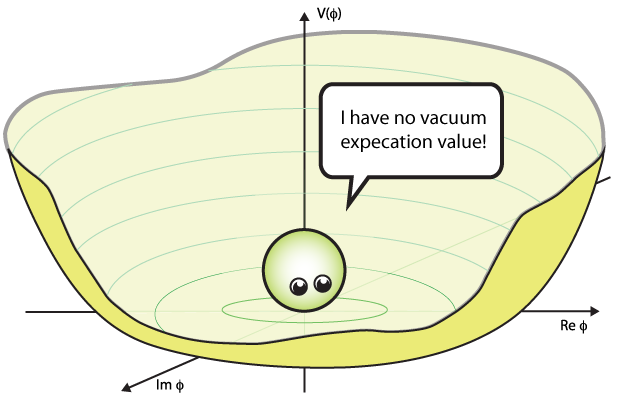
\includegraphics[width=0.5\textwidth]{chapter1/img/BoringPotential}
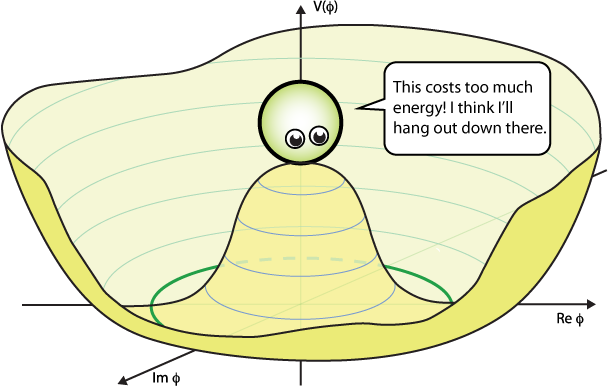
\includegraphics[width=0.5\textwidth]{chapter1/img/Higgs-Potential-lookdown}
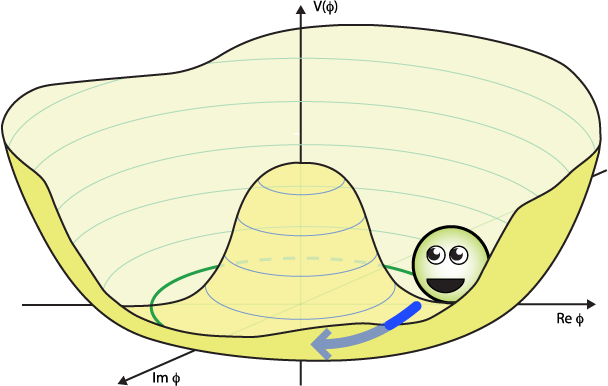
\includegraphics[width=0.5\textwidth]{chapter1/img/Higgs-Potential-Goldstone}
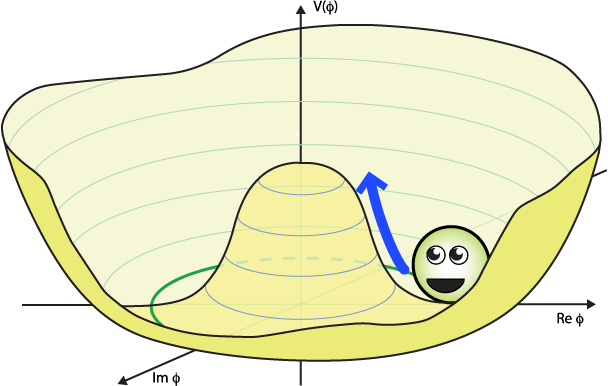
\includegraphics[width=0.5\textwidth]{chapter1/img/Higgs-Potential-radial}
\caption{In this example the Higgs potential is illustrated in function of a complex scalar field (2D). The principle is the same for a complex scalar doublet but a lot harder to visualize. \textit{Top left:} the Higgs potential with $\mu^2 > 0$, there is no vacuum expectation value. \textit{Top right:} $\mu^2 < 0$, the origin is now a maximum and not stable; the scalar field will move to the lowest possible energy state. \textit{Bottom left:} a flat direction in the potential corresponds to a massless Goldstone mode (remember there are two extra scalar fields in the full theory, meaning there are a total of three). \textit{Bottom right:} the concave shape of the potential near the minimum defines the Higgs boson mass. Illustrations from Ref. \cite{flip}.}
\label{fig:BEHpotential}
\end{figure}


\begin{equation}
\label{eq:zerominimum}
\langle 0|\Phi|0\rangle \equiv \Phi_0 = \begin{pmatrix} 0 \\ 0 \end{pmatrix}.
\end{equation} 
From Eq. \ref{eq:higgslagrangian} and \ref{eq:zerominimum}, one can see that the kinetic term does not give rise to massive particles in this scenario\footnote{Easy to see when substituting $v=0$ in Eq. \ref{eq:massesHiggs}.}. In the case of $\mu^2 < 0$, the minimum is no longer located at the origin of the fields: $\partial_{|\Phi|} V(|\Phi|) = 0$ for $|\Phi| = \sqrt{-\frac{\mu^2}{2\lambda}}$, hence one possible solution is\footnote{It is not possible for the charged part of the fields to have a vacuum expectation value as this would not be in agreement with electromagnetism. The upper part in Eq. \ref{eq:vev2} is therefore set to zero.}
\begin{equation}
\label{eq:vev2}
\langle 0|\Phi|0\rangle \equiv \Phi_0 = \begin{pmatrix} 0 \\ \frac{v}{\sqrt{2}} \end{pmatrix}, \ \ \textrm{with} \ \ v = \sqrt{-\frac{\mu^2}{\lambda}}.
\end{equation} 
$v$ is referred to as the \textit{vacuum expectation value} to reflect that the Higgs field is always ``on''. To investigate the terms, we can expand the field around the minimum:

\begin{equation}
\Phi(x) = \begin{pmatrix} \theta_2(x) + i\theta_1(x) \\ \frac{v+H(x)}{\sqrt{2}} - i\theta_3(x) \end{pmatrix} = e^{i\theta_a\tau_a}\begin{pmatrix} 0 \\ \frac{v+H(x)}{\sqrt{2}} \end{pmatrix}.
\end{equation}
Implementing this into Eq. \ref{eq:higgslagrangian} would yield the existence of unphysical fields $\phi_{1,2,3}$ that give rise to three extra degrees of freedom that were not present in the original Lagrangian\footnote{In Eq. \ref{eq:higgslagrangian}, the vector fields are massless and each give rise to 2 d.o.f. The vev makes the three vector fields massive, thus adding 3 d.o.f.\textit{and} introduce three unphysical fields.}. Since a change of variables cannot alter the number of d.o.f. of a system, one can conclude that three fields do not represent physical fields. They can be removed by fixing a gauge, the unitary gauge, that breaks the original symmetry of the system.
\begin{equation}
\label{eq:vev}
\Phi(x) \rightarrow e^{-i\theta_a\tau_a}\Phi(x) = \begin{pmatrix} 0 \\ \frac{v+H(x)}{\sqrt{2}} \end{pmatrix},
\end{equation}
where we have introduced a new scalar field $H(x)$. After inserting this in the kinetic part of the scalar Lagrangian (Eq. \ref{eq:higgslagrangian}) and redefining the gauge fields as

\begin{equation}
\begin{split}
W^\pm_\mu &= \frac{1}{\sqrt{2}}\left(W^1_\mu \mp iW^2_\mu\right),\\
Z_\mu &= \frac{1}{\sqrt{g^2 + g'^2}}\left(gW^3_\mu - g'B_\mu\right),\\
A_\mu &= \frac{1}{\sqrt{g^2 + g'^2}}\left(gW^3_\mu + g'B_\mu\right),
\end{split}
\end{equation}
we find for the kinetic part of the scalar Lagrangian:

\begin{equation}
|D_\mu\Phi|^2 = \frac{1}{2} \left(\partial_\mu H\right)^2 + \frac{1}{2}g^2\left(v+H\right)^2W^+_\mu W^{-\mu} + \frac{1}{8}\left(v+H\right)^2 \left(g^2 + g'^2\right)Z_\mu Z^\mu.
\end{equation}
Since mass terms enter this equation in the general form of $M^2_W W_\mu W^\mu$ for the $W$ bosons and $\frac{1}{2}M_Z^2 Z_\mu Z^\mu$ for the $Z$ boson, the mass terms of the gauge bosons after spontaneous symmetry breaking can be written down as:

\begin{equation}
\label{eq:massesHiggs}
\begin{split}
M_W &= \frac{1}{2}vg,\\
M_Z &= \frac{1}{2}v\sqrt{g^2+g'^2},\\
M_A &= 0,\\
\end{split}
\end{equation}
where it is clear that the photon remains massless\footnote{Because the $W$ and $Z$ bosons are massive, it costs energy to produce them and so the weak force is only really effective over a short distance. This is in contrast to the massless photons that result into a long range electomagnetic force. Thus, the Higgs field is responsible for the ``weakness'' of the weak force.}.\\


%\begin{corollary}[Eating the gauge bosons]
%A vev can give rise to massless Goldstone bosons. These particles correspond to the infinite possibilities of its phase in the potential. However, this would also lead to extra degrees of freedom in the Lagrangian. Therefore, one has to fix a gauge that results in the disappearance of the bosons and making the vector bosons of the original fields massive. 

%Specifically, the two massless $W^1, W^2$ bosons in the electroweak theory ($2 \times 2$ polarizations\footnote{A massless particle cannot have a third polarization, similar to a photon: it is traveling at the speed of light so it cannot have a polarization in the direction of propagation, only longitudinal.} = 4 d.o.f.) and two charged Higgses (2 d.o.f.) sum to a total of six degrees of freedom. In the broken theory, we have two massive $W^+,W^-$ bosons ($2 \times 3$ polarizations), which again total to six degrees of freedom.

%Similarly, the $W^3, B$ ($2\times2$ d.o.f.) and $H^0$ (2 d.o.f.) combine into the neutral $Z$ (massive, 3 d.o.f.), the $\gamma$ (2 d.o.f.) and the scalar $H$ (1 d.o.f.).

%Similar to the nucleons having a mass that is much greater than the summed mass of its constituents, the Higgs fields gives rise to the mass of these gauge bosons. In the case of nucleons, it is primarily the potential energy of the strong force that is responsible for the total mass following $E=mc^2$. The coupling of the gauge bosons to the Higgs field gives a sense of inertia to the particle. The particle does not float freely in vacuum but interacts with the ever present Higgs field (with a vev $\neq$ 0) making it massive.
%\end{corollary}

\noindent Using the potential term in Eq. \ref{eq:higgslagrangian} together with the vev in Eq. \ref{eq:vev}, we find for the Lagrangian of the Higgs boson
\begin{equation}
\mathcal{L}_H = \frac{1}{2}\left(\partial_\mu H\right)\left(\partial^\mu H\right) - \lambda v^2 H^2 - \lambda v H^3 - \frac{\lambda}{4}H^4.
\end{equation}
The first term again corresponds to the kinetic term, whereas the third and fourth refer to the three- and four-point self-interactions of the Higgs, respectively. Scalar masses have the general form $\frac{1}{2}m\phi^2$; the Higgs boson mass is thus equal to 

\begin{equation}
m_H = 2\lambda v^2 = - 2\mu^2,
\end{equation}
and needs to be determined experimentally.

Working through the interaction terms of the Lagrangian, one can show that the electric charge $e$  is related to the couplings of the weak isospin $g$ and hypercharge $g'$.

\begin{equation}
\label{eq:weinbergangle}
e = g \sin \theta_{W} = g' \cos \theta_W,
\end{equation} 
where the Weinberg angle is denoted as $\theta_W$ and indicates the magnitude of rotation of the boson fields after spontaneous symmetry breaking:

\begin{equation}
\begin{pmatrix} \gamma \\ Z \end{pmatrix} = 
\begin{pmatrix} \cos{\theta_W} & \sin{\theta_W} \\ -\sin{\theta_W} & \cos{\theta_W} \end{pmatrix} \begin{pmatrix} B^0 \\ W^0 \end{pmatrix},
\end{equation}
and is related to the weak isospin and hypercharge:

\begin{equation}
\cos \theta_W = \frac{g}{\sqrt{g^2 + g'^2}} \ \ \textrm{and} \ \ \sin \theta_W = \frac{g'}{\sqrt{g^2 + g'^2}}.
\end{equation}



\paragraph{Massive fermions}
A term like $-m\bar{\psi}\psi = -m\left[\bar{\psi}_L\psi_R + \bar{\psi}_R\psi_L\right]$, where we have decomposed the equation into the left- and right-handed chiral states\footnote{$\psi_L = P_L \psi = \frac{1-\gamma^5}{2} \psi$ and $\psi_R = P_R \psi = \frac{1+\gamma^5}{2} \psi$.} is not gauge invariant in the Lagrangian. The left-handed fermions form an isospin \textit{doublet} and the right-handed fermions form isospin \textit{singlets}. They transform differently under SU(2)$_L \times$ U(1)$_Y$:
\begin{equation}
\begin{split}
\chi_L &\rightarrow \chi'_L = \chi_L e^{i \vec{\tau_L} \vec{W}+i\alpha Y_W},\\
\psi_R &\rightarrow \psi'_R = \psi_R e^{i\alpha Y_W}.\\
\end{split}
\end{equation} 
It is possible for the fields to couple to the complex Higgs doublet, defined in Eq. \ref{eq:higgsdoublet}, by adding Yukawa couplings. This results into terms that are singlets under SU(2)$_L$ and U(1)$_Y$:

\begin{equation}
\label{eq:yukawa}
\mathcal{L}_{Yuk} = \lambda_e \overline{L_L}\Phi e_R - \lambda_d \overline{Q_L} \Phi d_R - \lambda_u \overline{Q_L} \tilde{\Phi}u_R + h.c.,
\end{equation}
where we have introduced the conjugate of $\Phi,\tilde{\Phi} = i\tau_2 \Phi^*$, which has a negative hypercharge. After spontaneous symmetry breaking (Eq. \ref{eq:vev}), we find:

\begin{equation}
\begin{split}
L_{Yuk} &= -\frac{1}{\sqrt{2}} \lambda_e \left(\bar{\nu}_e, \bar{e}_L\right) \begin{pmatrix} 0 \\ v+H(x) \end{pmatrix} e_R + ... \\
\ &= -\frac{1}{\sqrt{2}} \lambda_e \left(v+H(x)\right)\bar{e}_L e_R + ...,
\end{split}
\end{equation}
where we highlighted only the electron part. Fermion mass terms have the general form $m_f \bar{f}_L f_R$ + h.c.. Therefore, one finds:

\begin{equation}
m_e = \frac{\lambda_e v}{\sqrt{2}}, \ \ \ m_u = \frac{\lambda_u v}{\sqrt{2}}, \ \ \ m_d = \frac{\lambda_d v}{\sqrt{2}}.
\end{equation}
The mass of the fermions is again not predicted since the Yukawa coupling parameters are free parameters. 

\subsection{Particle mixing}
\label{subsec:particlemixing}
%THIS IS GONE
\iffalse
In Eq. \ref{eq:yukawa}, we introduced Yukawa coupling constants to explain the mass of fermions. In its most general realizations, these couplings are not constants but matrices. This will introduce possible mixing of \textit{flavor eigenstates} into different \textit{mass eigenstates}. Let us write out the first term in Eq. \ref{eq:yukawa}:

\begin{equation}
\begin{split}
\lambda_e \overline{L_L} \Phi e_R &= \Lambda^e_{ij}\overline{L^I_{Li}} \Phi e^I_{Rj} = \Lambda^e_{ij}\overline{\left(\textrm{neutral leptons, charged leptons}\right)^I_{Li}} \begin{pmatrix} \phi^+ \\ \phi^0 \end{pmatrix}  \left(\textrm{charged leptons}\right)^I_{Rj} \\
&= \begin{pmatrix} 
\Lambda_{11}\overline{\left(\nu_e \ e\right)^I_L}\begin{pmatrix} \phi^+ \\ \phi^0 \end{pmatrix} &
\Lambda_{12}\overline{\left(\nu_e \ e\right)^I_L}\begin{pmatrix} \phi^+ \\ \phi^0 \end{pmatrix} &
\Lambda_{13}\overline{\left(\nu_e \ e\right)^I_L}\begin{pmatrix} \phi^+ \\ \phi^0 \end{pmatrix}\\  
\Lambda_{21}\overline{\left(\nu_\mu \ \mu\right)^I_L}\begin{pmatrix} \phi^+ \\ \phi^0 \end{pmatrix} &
\Lambda_{22}\overline{\left(\nu_\mu \ \mu\right)^I_L}\begin{pmatrix} \phi^+ \\ \phi^0 \end{pmatrix} &
\Lambda_{23}\overline{\left(\nu_\mu \ \mu\right)^I_L}\begin{pmatrix} \phi^+ \\ \phi^0 \end{pmatrix}\\
\Lambda_{31}\overline{\left(\nu_\tau \ \tau\right)^I_L}\begin{pmatrix} \phi^+ \\ \phi^0 \end{pmatrix} &
\Lambda_{32}\overline{\left(\nu_\tau \ \tau\right)^I_L}\begin{pmatrix} \phi^+ \\ \phi^0 \end{pmatrix} &
\Lambda_{33}\overline{\left(\nu_\tau \ \tau\right)^I_L}\begin{pmatrix} \phi^+ \\ \phi^0 \end{pmatrix}
\end{pmatrix}
\cdot \begin{pmatrix} e^I_R \\ \mu^I_R \\ \tau^I_R \end{pmatrix},
\end{split}
\end{equation}
where the superscript $I$ implies that the fermion fields are expressed in the \textit{interaction (flavor)} basis. The subscript $i$ stands for the three generations.

This means that after symmetry breaking the lepton mass terms break down into

\begin{equation}
\label{eq:yukawaleptons}
\begin{split}
-\mathcal{L}^{\textrm{leptons}}_{Yuk} &= \Lambda^\nu_{ij}\overline{\nu^I_{Li}} \frac{v}{\sqrt{2}}\nu^I_{Rj} + ...\\
&= M^\nu_{ij} \overline{\nu^I_{Li}} \nu^I_{Rj} + ...
\end{split}
\end{equation}
where we have omitted the hermitian conjugate terms and the Higgs field interaction terms. Note that the $l$-term in the equation still represents the three lepton types. There is mixing between the flavor fields as there is no reason why the matrix $M$ should be diagonal\footnote{The question and answer of flavor/mass mixing can be put as: Q: ``Why is there mixing?''; A: ``Because it can.''}.

To obtain proper mass terms, one has to diagonalize the mass matrix $M^l$ and find proper eigenstates. We introduce unitary matrix $U$ as follows

\begin{equation}
M^l_{diag} = U^l_L M^l U^{l\dagger}_R,
\end{equation}
which can be done when the matrix $V$ are unitary $\left(U^{l\dagger}_L U^{l}_L = \mathbbm{1}\right)$. Eq. \ref{eq:yukawaleptons} can now be expressed as follows:

\begin{equation}
\begin{split}
-\mathcal{L}^{\textrm{leptons}}_{Yuk} &= \overline{l^I_{Li}} M^l_{ij} l^I_{Rj} + ...\\
&= \overline{l^I_{Li}} U^{l\dagger}_L U^l_L M^l_{ij} U^{l\dagger}_R U^{l}_R l^I_{Rj} ...\\
&= \overline{l_{Li}} \left(M^l_{ij}\right)_{diag} l_{Rj} + ...,
\end{split}
\end{equation}
where the $U$ matrices have been absorbed in the lepton flavor eigenstates and have formed mass eigenstates. These mass eigenstates couple differently to the gauge fields of the weak interaction. Working out one term from Eq. \ref{eq:EW}, the mixing of the flavor eigenstates is clearly visible

\begin{equation}
\begin{split}
\mathcal{L}_{kinetic}\left(L_L\right) &= i\overline{L^I_{Li}}\gamma_\mu D^\mu L^I_{Li} \\
&= \frac{g}{\sqrt{2}}\overline{\nu^I_{Li}} \gamma_\mu W^{-\mu} l^I_{Li} + \frac{g}{\sqrt{2}} \overline{l^I_{Li}} \gamma_\mu W^{+\mu} \nu^I_{Lj} + ...\\
&= \frac{g}{\sqrt{2}}\overline{\nu_{Li}} \left(U^{l\dagger}_L\right)_{ij} \gamma_\mu W^{-\mu} l_{Lj} + \frac{g}{\sqrt{2}} \overline{l_{Li}} \left(U^l\right)_{ij} \gamma_\mu W^{+\mu} \nu_{Lj} + ...\\
\end{split}
\end{equation}
The matrix $U$ is known as the \textit{Pontecorvo-Maki-Nakagawa-Sakata (PMNS)} mixing matrix \cite{doi:10.1143/PTP.28.870}. The interaction and mass eigenstates can differ and the rotation is given by

\begin{equation}
\nu^I_i = U_{PMNS} \nu_i,
\end{equation}
or explicitly:


\begin{equation}
\begin{split}
\begin{pmatrix} \nu_e \\ \nu_\mu \\ \nu_\tau \end{pmatrix} = 
\begin{pmatrix} 
U_{e1} & U_{e2} & U_{e3} \\
U_{\mu 1} & U_{\mu 2} & U_{\mu 3} \\
U_{\tau 1} & U_{\tau 2} & U_{\tau 3}
\end{pmatrix}
\begin{pmatrix} \nu_1 \\ \nu_2 \\ \nu_3 \end{pmatrix}.
\end{split}
\end{equation}
Because the choice of the global phases of the lepton fields is arbitrary and the matrix is unitary, the nine unknown complex elements can be reduced to three real numbers and one phase\footnote{This phase is responsible for \textit{CP-violation.}}. The matrix is most often written as:

\begin{equation}
\mathcal{U} = \begin{pmatrix}
1 	& 0 		& 0 \\
0 	& c_{23}	& s_{23} \\
0	& -s_{23} 	& c_{23}
\end{pmatrix}
\begin{pmatrix}
c_{13} 				& 0 		& s_{13}e^{-i\delta} \\
0 					& 1			& 0 \\
s_{13}e^{-i\delta}	& 0 		& c_{13}
\end{pmatrix}
\begin{pmatrix}
c_{12} 	& s_{12}	& 0 \\
-s_{12} & c_{12}	& 0 \\
0		& 0			& 1
\end{pmatrix}
\cdot \textrm{diag}\left(e^{i\alpha_1/2},e^{i\alpha_2/2},2\right).
\end{equation}


\noindent Without going into detail, it is worth noting that a similar matrix exists that connects the quark flavor and mass eigenstates. In contrast to the leptons, the up-type interaction doublet states are chosen to be the same as the mass eigenstates. The mixing of the mass and interaction eigenstates is in the down-type sector. This matrix is known as the \textit{Cabibbo...} mixing matrix, 


\begin{equation}
V_{CKM} = \begin{pmatrix}
c_{12}c_{13} & s_{12}c_{13} & s_{13}e^{-i\delta} \\
-s_{12}c_{23} - c_{12}s_{23}s_{13} e^{i\delta} & c_{12}c_{23} - s_{12}s_{23}s_{13}e^{i\delta} & s_{23}c_{13} \\
s_{12}s_{23} - c_{12}c_{23}s_{13}e^{i\delta} 
& -c_{12}s_{23} - s_{12}c_{23}s_{13}e^{i\delta} & c_{23}c_{13}
\end{pmatrix},
\end{equation}
where $c_{ij} = \cos\left(\theta_{ij}\right)$ and  $s_{ij} = \sin\left(\theta_{ij}\right)$ for $i<j = 1,2,3$ and $\delta$ is the $CP$-violating phase.

\noindent The mixing of the flavor quantum states is necessary to explain charged current interactions changing the strangeness with one \cite{Glashow:1970gm} and $CP$-violating processes \cite{1964PhRvL}.
\fi
%GONE UP TO HERE

In Eq. \ref{eq:yukawa}, we introduced Yukawa coupling constants to explain the mass of fermions. In its most general realizations, these couplings are not constants but matrices. This will introduce possible mixing of \textit{flavor eigenstates} into different \textit{mass eigenstates}. Let us write out the second term in Eq. \ref{eq:yukawa}:

\begin{equation}
\begin{split}
\lambda_d \overline{Q_L} \Phi d_R &= \Lambda^d_{ij}\overline{Q^I_{Li}} \Phi d^I_{Rj} = \Lambda^d_{ij}\overline{\left(\textrm{up-type down-type}\right)^I_{Li}} \begin{pmatrix} \phi^+ \\ \phi^0 \end{pmatrix}  \left(\textrm{down-type}\right)^I_{Rj} \\
&= \begin{pmatrix} 
\Lambda_{11}\overline{\left(u \ d\right)^I_L}\begin{pmatrix} \phi^+ \\ \phi^0 \end{pmatrix} &
\Lambda_{12}\overline{\left(u \ d\right)^I_L}\begin{pmatrix} \phi^+ \\ \phi^0 \end{pmatrix} &
\Lambda_{13}\overline{\left(u \ d\right)^I_L}\begin{pmatrix} \phi^+ \\ \phi^0 \end{pmatrix}\\  
\Lambda_{21}\overline{\left(c \ s\right)^I_L}\begin{pmatrix} \phi^+ \\ \phi^0 \end{pmatrix} &
\Lambda_{22}\overline{\left(c \ s\right)^I_L}\begin{pmatrix} \phi^+ \\ \phi^0 \end{pmatrix} &
\Lambda_{23}\overline{\left(c \ s\right)^I_L}\begin{pmatrix} \phi^+ \\ \phi^0 \end{pmatrix}\\
\Lambda_{31}\overline{\left(t \ b\right)^I_L}\begin{pmatrix} \phi^+ \\ \phi^0 \end{pmatrix} &
\Lambda_{32}\overline{\left(t \ b\right)^I_L}\begin{pmatrix} \phi^+ \\ \phi^0 \end{pmatrix} &
\Lambda_{33}\overline{\left(t \ b\right)^I_L}\begin{pmatrix} \phi^+ \\ \phi^0 \end{pmatrix}
\end{pmatrix}
\cdot \begin{pmatrix} d^I_R \\ s^I_R \\b^I_R \end{pmatrix},
\end{split}
\end{equation}
where the superscript $I$ implies that the fermion fields are expressed in the \textit{interaction (flavor)} basis. The subscript $i$ stands for the three generations. This means that after symmetry breaking the quark mass terms break down into

\begin{equation}
\label{eq:yukawaquarks}
\begin{split}
-\mathcal{L}^{\textrm{quarks}}_{Yuk} &= \Lambda^d_{ij}\overline{d^I_{Li}} \frac{v}{\sqrt{2}}d^I_{Rj} + \Lambda^u_{ij} \overline{u^I_{Li}} \frac{v}{\sqrt{2}} u^I_{Rj} + ...\\
&= M^d_{ij} \overline{d^I_{Li}} d^I_{Rj} + M^u_{ij} \overline{u^I_{Li}} u^I_{Rj} + ...
\end{split}
\end{equation}
where we have omitted the hermitian conjugate terms and the Higgs field interaction terms. Note that the $u$- and $d$-terms in the equation still each represent the three up- and down-type quarks repectively. There is mixing between the flavor fields as there is no reason why the matrix $M$ should be diagonal\footnote{The question and answer of flavor/mass mixing can be put as: Q: ``Why is there mixing?''; A: ``Because it's possible.''}.

To obtain proper mass terms, one has to diagonalize the mass matrices $M^u$ and $M^d$ and find proper eigenstates. We introduce unitary matrices $V$ as follows

\begin{equation}
\begin{split}
M^d_{diag} &= V^d_L M^d V^{d\dagger}_R,\\
M^u_{diag} &= V^u_L M^u V^{u\dagger}_R,
\end{split}
\end{equation}
which can be done when the matrices $V$ are unitary $\left(V^{d,u\dagger}_L V^{d,u}_L = \mathbbm{1}\right)$. Eq. \ref{eq:yukawaquarks} can now be expressed as follows:

\begin{equation}
\begin{split}
-\mathcal{L}^{\textrm{quarks}}_{Yuk} &= \overline{d^I_{Li}} M^d_{ij} d^I_{Rj} + \overline{u^I_{Li}} M^u_{ij} u^I_{Rj} + ...\\
&= \overline{d^I_{Li}} V^{d\dagger}_L V^d_L M^d_{ij} V^{d\dagger}_R V^{d}_R d^I_{Rj} + \overline{u^I_{Li}} V^{u\dagger}_L V^u_L M^u_{ij} V^{u\dagger}_R V^u_R u^I_{Rj} + ...\\
&= \overline{d_{Li}} \left(M^d_{ij}\right)_{diag} d_{Rj} + \overline{u_{Li}} \left(M^u_{ij}\right)_{diag} u_{Rj} + ... \\,
\end{split}
\end{equation}
where the $V$ matrices have been absorbed in the quark flavor eigenstates and have formed mass eigenstates. These mass eigenstates couple differently to the gauge fields of the weak interaction. Working out one term from Eq. \ref{eq:EW}, the mixing of the flavor eigenstates is clearly visible

\begin{equation}
\begin{split}
\mathcal{L}_{kinetic}\left(Q_L\right) &= i\overline{Q^I_{Li}}\gamma_\mu D^\mu Q^I_{Li} \\
&= \frac{g}{\sqrt{2}}\overline{u^I_{Li}} \gamma_\mu W^{-\mu} d^I_{Li} + \frac{g}{\sqrt{2}} \overline{d^I_{Li}} \gamma_\mu W^{+\mu} u^I_{Li} + ...\\
&= \frac{g}{\sqrt{2}}\overline{u_{Li}} \left(V^u_L V^{d\dagger}_L\right)_{ij} \gamma_\mu W^{-\mu} d_{Lj} + \frac{g}{\sqrt{2}} \overline{d_{Li}} \left(V^d V^{u\dagger}\right)_{ij} \gamma_\mu W^{+\mu} u_{Lj} + ...\\
\end{split}
\end{equation}
The combination of matrices $\left(V^d_L V^{u\dagger}_L\right)_{ij}$, a unitary $3 \times 3$ matrix is known as the \textit{Cabibbo-Kobayashi-Maskawa (CKM)} mixing matrix. By convention, the interaction and flavor eigenstates of the up-type quarks are chosen to be equal. The down-type quarks are therefore chosen to be rotated:

\begin{equation}
\begin{split}
u^I_i &= u_i,\\
d^I_i &= V_{CKM} d_i,
\end{split}
\end{equation}
or explicitly:


\begin{equation}
\begin{split}
\begin{pmatrix} d^I \\ s^I \\ b^I \end{pmatrix} = 
\begin{pmatrix} 
V_{ud} & V_{us} & V_{ub} \\
V_{cd} & V_{cs} & V_{cb} \\
V_{td} & V_{ts} & V_{tb}
\end{pmatrix}
\begin{pmatrix} d \\ s \\ b \end{pmatrix}.
\end{split}
\end{equation}
Because the choice of the global phases of the quark fields is arbitrary and the matrix is unitary, the nine unknown complex elements can be reduced to three real numbers and one phase\footnote{This phase is responsible for \textit{CP-violation.}}. The matrix is most often written as:


\begin{equation}
V_{CKM} = \begin{pmatrix}
c_{12}c_{13} & s_{12}c_{13} & s_{13}e^{-i\delta} \\
-s_{12}c_{23} - c_{12}s_{23}s_{13} e^{i\delta} & c_{12}c_{23} - s_{12}s_{23}s_{13}e^{i\delta} & s_{23}c_{13} \\
s_{12}s_{23} - c_{12}c_{23}s_{13}e^{i\delta} 
& -c_{12}s_{23} - s_{12}c_{23}s_{13}e^{i\delta} & c_{23}c_{13}
\end{pmatrix},
\end{equation}
where $c_{ij} = \cos\left(\theta_{ij}\right)$ and  $s_{ij} = \sin\left(\theta_{ij}\right)$ for $i<j = 1,2,3$ and $\delta$ is the $CP$-violating phase.

The mixing of the flavor quantum states is necessary to explain charged current interactions changing the strangeness with 1 \cite{Glashow:1970gm} and $CP$-violating processes \cite{1964PhRvL}.\\

\noindent Without going into detail, it is worth noting that a similar matrix exists that connects the lepton flavor and mass eigenstates. In contrast to the quarks, the down-type interaction doublet states are chosen to be the same as the mass eigenstates. Therefore, the mixing of the mass and interaction eigenstates is in the neutrino sector. The three eigenstates of the weak interaction form an orthonormal basis. Left-handed neutrinos and leptons form doublets $L$ as can be seen in Eq. \ref{eq:yukawa}: $\begin{pmatrix}\nu_e \\ e \end{pmatrix}$, $\begin{pmatrix}\nu_\mu \\ \mu \end{pmatrix}$ and $\begin{pmatrix}\nu_\tau \\ \tau \end{pmatrix}$. One can also construct an eigenbasis out of three neutrino states with of definite mass, $\nu_1, \nu_2$ and $\nu_3$ that diagonalize the neutrino's free-particle Hamiltonian. Similar to quarks, this mass-eigenbasis is rotated relative to the flavor-eigenbasis:

\begin{equation}
\begin{pmatrix}
\nu_e \\ \nu_\mu \\ \nu_\tau
\end{pmatrix}
=
\begin{pmatrix}
U_{e1} & U_{e2} & U_{e3} \\
U_{\mu 1} & U_{\mu 2} & U_{\mu 3} \\
U_{\tau 1} & U_{\tau 2} & U_{\tau 3} \\
\end{pmatrix}
\begin{pmatrix}
\nu_1 \\ \nu_2 \\ \nu_3
\end{pmatrix}
\end{equation}

\noindent This matrix is known as the Pontecorvo-Maki-Nakagawa-Sakata (PMNS) matrix \cite{doi:10.1143/PTP.28.870},

\begin{equation}
\mathcal{U} = \begin{pmatrix}
1 	& 0 		& 0 \\
0 	& c_{23}	& s_{23} \\
0	& -s_{23} 	& c_{23}
\end{pmatrix}
\begin{pmatrix}
c_{13} 				& 0 		& s_{13}e^{-i\delta} \\
0 					& 1			& 0 \\
s_{13}e^{-i\delta}	& 0 		& c_{13}
\end{pmatrix}
\begin{pmatrix}
c_{12} 	& s_{12}	& 0 \\
-s_{12} & c_{12}	& 0 \\
0		& 0			& 1
\end{pmatrix}
\end{equation}
%\cdot \textrm{diag}\left(e^{i\alpha_1/2},e^{i\alpha_2/2},2\right).

\noindent The matrix is again parameterized by three mixing angles $\theta_{12}, \theta_{13}$ and $\theta_{23}$ where $s_{ij}$ and $c_{ij}$ are used to denote $\sin\left(\theta_{ij}\right)$ and $\cos\left(\theta_{ij}\right)$. The phase $\delta$ relates to charge-parity violations. It is possible to add additional ``Majorana'' phases, but this will not be discussed in this work \cite{Giganti:2017fhf}.
 
\section{A success story}
Over the course of multiple decades, the Standard Model was built up into an extremely comprehensive theory. The first building blocks necessary for its construction came from experiments in the early 20th century when its quantum characteristics became more apparent. The theory was formulated as a gauge theory in the 1960s and 1970s and for decades it has been rigorously tested and checked, leading to extremely accurate experimental precision measurements that agree with the theory. Apart from precision measurements, it has led to predictions of particles and their interactions, which could only be tested years or decades after they were first proposed. In the following, we give a brief overview of some experimental results.

\iffalse
\subsection{Wave-particle duality}
One of the most striking features of the SM is that particles may be partly described in terms of not only particles, but also of waves. The classical concepts of ``particles'' or ``waves'' is insufficient in describing the behaviour of quantum-scale objects. In the late 18th and early 19th century, physicist were puzzled by the successful approaches to well known problems of electromagnetic phenomena, which were widely accepted as fields, with quantizations (particles). Black body radiation and the photoelectric effect are described below. In quantum field theory, particles are defined as excited states of a field. The wave-nature is evident in the calculated \textit{probability distributions} for a given reaction.

\subsubsection{Photoelectric effect}
At the close of the 19th century, J.J. Thomson found that electricity is caused by \textit{particles} that can fly through vacuum. But, since electromagnetism was known to be a wave that is generated by a changing electric or magnetic \textit{field}, a particle description of electricity and charge was, in a way, flawed by construction. 
A first step towards quantization came when the ultraviolet catastrophe seemed to be solved if black-body radiation is not explained by the classical equipartition theorem (Appendix \ref{ch:planck}), but a quantization of the electromagnetic field: Planck's law. Planck denounced these particles of light as a limitation of his approximation, not a property of reality. It was only later, when Einstein combined this theory with the photoelectric effect, that light quanta/photons became more accepted.

The potoelectric effect describes that when a material is shined upon by light, electrons or other free carriers can be emitted. In a classical theory perspective, an alteration in the intensity of light would induce changes in the kinetic energy of the particles emitted from the material. Instead, these particles are dislodged only by the impingement of photons when those photons reach or exceed a threshold frequency/energy. Changing the intensity of the light bundle only changes the amount of particles released, but does not alter its kinetic energy. This is easy to explain in a quantum view and resulted in the Einstein's Nobel Prize in 1921.

\subsubsection{Double-slit experiment}
%https://www.physics.umd.edu/courses/Phys401/appeli/EXTRAS/double-slitexperiment.pdf
The double-slit experiment was first performed by Thomas Young in the early 19th century. If a beam of light shines through two slits of a screen onto a second screen behind the first, an interference pattern can be seen as illustrated in Figure \ref{fig:doubleslit}. This proved the wavelike nature of light.

\begin{figure}
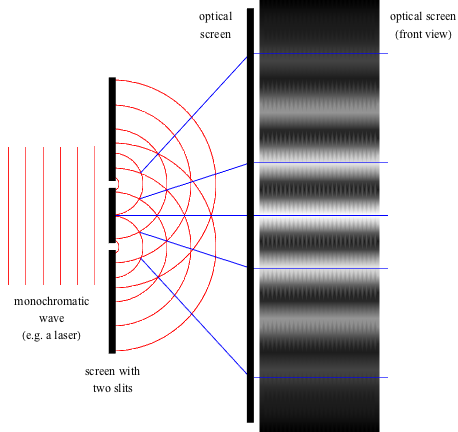
\includegraphics[width=0.6\textwidth,height=0.5\linewidth]{chapter1/img/younginterference.png}
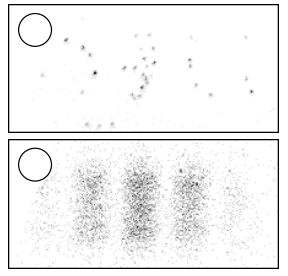
\includegraphics[width=0.4\textwidth,height=0.5\linewidth]{chapter1/img/doubleslitsinglephoton_crop.png}
\caption{\textit{Left:} Schematic view of interference pattern as in Young's experiment \cite{shmoop}.  \textit{Right:} (top) a single 20 ms time frame showing several individual photon arrival points; (bottom) image obtained after integrating for a few seconds: the diffraction pattern emerges \cite{weiswynands:2003}. }
\label{fig:doubleslit}
\end{figure}

In later years, similar experiments for electrons were done to prove the wavelike properties of particles \cite{Davisson:1927ta,thomson:1927}. The same double-slit experiment was finally perfomed in the 60s \cite{Jonsson1961} and for single electrons in 1974 \cite{merli:1974}. Single photon \cite{weiswynands:2003} (shown in Figure \ref{fig:doubleslit}) and single electron double-slit experiments show the same results, illustrating the wave probability interpretation of particles and fields.
\fi

\subsection{Predictions}
By 1932, scientists knew that atoms were made up by protons, neutrons and electrons. Together with the photon, a total number of four particles were known. Four grew to five when Anderson discovered the existence of positrons \cite{Anderson:1933mb} (predicted by Dirac \cite{Dirac:1928hu}). Then came the muon \cite{Neddermeyer:1937md} and pion \cite{Lattes:1947mw}. By the 1960s, there were ``fundamental particles'' with no good guiding principles to link them together. They were often referred to as the ``particle zoo''.

By a series of insights by several individuals, the Standard Model as a quantum field theory became more widely accepted. Since then, the model has predicted the results of experiment after experiment. Some of them are:

\vspace{2mm}

\begin{itemize}
\item Neutral weak currents. Postulated by Salam, Weinberg and Glashow, the theory of electroweak interactions predicted the existence of a new type of weak interaction, in which the reacting particles do not change their charges. The first observation was made in 1973 in the Gargamelle experiment at the European nuclear research laboratory, CERN \cite{Hasert:1973ff}.
\item Weak gauge bosons. Again postulated by the abovementioned people. These particles were discovered in the UA1 and UA2 experiments in CERN, 1983 \cite{Arnison:1983rp,Arnison:1983mk}.
\item Heavy quarks. To explain the $CP$-violations in kaon decays, M. Kobayashi and T. Maskawa predicted the existence of a third generation of quarks: the \textit{top} and \textit{bottom} quarks. The bottom quark was discovered in 1977 at Fermilab \cite{Herb:1977ek}. It took another 18 years for the top quark to be found in the same institute \cite{Abe:1995hr}. 
\item Gluons. The gauge bosons of quantum chromodynamics were discovered in 1978 and 1979 \cite{Barber:1979yr}.
\item Higgs boson. On July 4, 2012, physicists at CERN announced the discovery of the only fundamental particle predicted by the Standard Model that was not yet discovered. 
\end{itemize}  
\subsection{Precision tests}
%Below, a small subset of many precision tests is given: 

%\begin{itemize}
%\item \textit{Lamb shift}, a difference in energy between two energy levels of the hydrogen atom that was not predicted by the Dirac equation. This phenomenon is explained with the theory of QED. \textcolor{red}{REF}.
%\item \textcolor{red}{Andere goede voorbeelden? Precision measurements in IceCube? vb: Neutrino cross-section: IceCube/Nature https://www.nature.com/articles/nature24459}

%\end{itemize}

Inconsistencies between experiment and theory can be signs of wrong or incomplete theories. For this reason, experimentalists are continuously testing parameters of the SM. These precision tests are most often done by testing the theory of quantum electrodynamics (QED). With the use of \textit{renormalization theory}, many parameters of the theory can be calculated with high precision. High-precision measurements of various observables have been performed at LEP 1 and SLC \cite{ALEPH:2005ab,Riemann:2010zz,Abe:2000dq,Abe:2000uc,Abe:2000hk,Abe:1996ef} for physics at the $Z$-boson mass ($\sqrt{s} \approx M_Z$) and other observables at Tevatron \cite{Aaltonen:2013iut,TEW:2010aj}, LEP 2 \cite{TEW:2010aj}, ATLAS \cite{Aaboud:2017svj,ATLASurl1} and CMS \cite{CMSurl1,CMSurl2}. Some of them are listed in Table \ref{tab:precision}. The parameters in the table show that the SM best-fit predictions are very consistent with what we see in experiments.

\vspace{2mm}
\begin{itemize}
\item The SM predicts kaons to decay into charged pions and a neutrino-antineutrino pair to happen once every ten billion kaon decays. The SM fit to this decay has a small uncertainty, making the search interesting for possible anomalies. A candidate event of this very rare decay has been reported by the NA62 collaboration in 2018 but is in accordance with the SM predictions \cite{na62}.

\item Another example is the measurement of the \textit{Lamb shift}, a difference in energy between two energy levels of the hydrogen atom that was not predicted by the Dirac equation and currently provides a measurement of the fine-structure constant $\alpha$ to better than one part in a million, allowing a precision test of QED.

\item Electrons have a magnetic dipole moment as a result from their intrinsic spin. A charge distribution in these particles, which we do not expect to happen for fundamental particles, would make the electon charge not seem perfectly spherical. This electron electric dipole moment (EDM) is expected from the SM only with an extremely small value from radiative corrections with $CP$-violating interactions, at most $10^{-38}\ e \cdot \textrm{cm}$. Recent measurements from the ACME experiment set the current upper limit at a value of  $1.1 10^{-29}\ e \cdot \textrm{cm}$ \cite{Cesarotti:2018huy}.
\end{itemize}
\vspace{2mm}

\noindent There have been other, more challenging precision test, such as neutrino cross-section measurements \cite{Aartsen:2017kpd} and measurements of the top quark mass in the CMS experiment \cite{Castro:2017yxe}. Both are again in agreement with the SM.


\begin{table}[]
\centering
\caption{Observables compared with the SM best fit. Errors are the total (experimental plus theoretical) uncertainties. Results are taken from Tables 10.4 and 10.5 in \cite{PDG2018url}.}
\label{tab:precision}
\resizebox{\textwidth}{!}{%
\begin{tabular}{|l|c|c|c|}
\hline
\rowcolor[HTML]{F1A91E} \textbf{Parameter}                                                 & \textbf{Experimental value}                              & \textbf{Theoretical value}                               & \textbf{Standard deviation} \\ \hline
$m_t$ {[}GeV{]}                                           & $172.74 \pm 0.46$                               & $172.96 \pm 0.45$                               & -0.5              \\ \hline
                  & $80.387 \pm 0.016$                              & \multirow{3}{*}{$80.358 \pm 0.004$}             & 1.8               \\ \cline{2-2} \cline{4-4}
                                                  & $80.376 \pm 0.033$                              &                                                 & 0.6               \\ \cline{2-2} \cline{4-4}
\multirow{-3}{*}{$m_W$ {[}GeV{]}}                                  & $80.370 \pm 0.019$                              &                                                 & 0.6               \\ \hline
            & $2.046 \pm 0.049$                               & \multirow{2}{*}{$2.089 \pm 0.001$}              & -0.9              \\ \cline{2-2} \cline{4-4}
  \multirow{-2}{*}{$\Gamma_W$ {[}GeV{]}}       & $2.195 \pm 0.083$                               &                                                 & 1.3               \\ \hline
$m_H$ {[}GeV{]}                                   & $125.14 \pm 0.15$                                                 & $125.14 \pm 0.15$                               & 0.0               \\ \hline
$g^{\nu e}_V$                                             & $-0.040 \pm 0.015$                              & $-0.0398 \pm 0.0001$                            & 0.0               \\ \hline
$g^{\nu e}_A$                                             & $-0.507 \pm 0.014$                              & $-0.5063$                                       & 0.0               \\ \hline
$\tau_\tau$ {[}fs{]}                                      & $290.75 \pm 0.36$                               & $290.39 \pm 2.17$                               & 0.1               \\ \hline
$\frac{1}{2}\left(g_\mu - 2 - \frac{\alpha}{\pi} \right)$ & $\left( 4511.18 \pm 0.77\right) \times 10^{-9}$ & $\left(4508.63 \pm 0.03 \right) \times 10^{-9}$ & 3.3               \\ \hline
$M_Z$ {[}GeV{]}                                           & $91.1876 \pm 0.0021$                            & $91.1884 \pm 0.0020$                            & -0.4              \\ \hline
$\Gamma_Z$ {[}GeV{]}                                      & $2.4952 \pm 0.0023$                             & $2.4942 \pm 0.0008$                             & 0.4               \\ \hline
$\Gamma_Z (\textrm{had})$ {[}GeV{]}                                & $1.7444 \pm 0.0020$                             & $1.7411 \pm 0.0008$                             & -                 \\ \hline
$\Gamma_Z (\textrm{inv})$ {[}MeV{]}                                & $499.0 \pm 1.5$                                 & $501.44 \pm 0.04$                               & -                 \\ \hline
$\Gamma_Z \left(l^+ l^- \right)$ {[}MeV{]}                & $83.984 \pm 0.086$                              & $83.959 \pm 0.008$                              & -                 \\ \hline
\end{tabular}%
}
\end{table}



\section{The need for physics beyond the Standard Model}
\label{needforBSM}
Despite its incredible success, many physicists believe the Standard Model is certainly not the full story. There are a number of features that seem arbitrary, but also some that cannot be explained by the theory alone. Below, I give a list of open questions:

\vspace{2mm}

\begin{itemize}
\item Why are there \textbf{three families} for both leptons and quarks? Why  not two? Or four? Or even a thousand?
\item What is the \textbf{cause of the symmetries} we see in the Standard Model? Why is, for example, QCD not an SU(4) gauge theory?
\item There are a number of \textbf{parameters} in the SM that cannot be explained by first principles. We have no good explanation for why the top quark is 75 000 times heavier than the up quark. Why is the vev of the Higgs potential 246 GeV? Why is the Higgs mass 125 GeV? There are in total 26 parameters in the SM that are determined by experiments and can be found in Table \ref{tab:freeparameters}.
\item Why does the Higgs potential have this\textbf{ Mexican hat shape}? In other words, why is $\mu^2$ in $\lambda \left(\Phi^\dagger \Phi \right)^2 + \mu^2\left(\Phi^\dagger \Phi \right)$ negative? Also, the vev, the mass of the Higgs boson and the mass of the fermions due to the Yukawa couplings all appear in Table \ref{tab:freeparameters}. This makes us believe there is something we do not fully understand about the BEH mechanism. 
\item Right-handed neutrinos can be introduced into the SM. They are singlets with respect to the strong and weak interaction and would therefore not carry an electric charge, weak hypercharge or weak isospin. Due to this lack of charge, right-handed neutrinos would be extremely difficult to detect. They have Yukawa interactions with other leptons and the Higgs boson, but its coupling would be extremely small. Neutrinos can become massive with Dirac mass terms in the same way charged leptons become massive in the BEH mechanism. Their \textbf{extremely small masses} suggest another mechanism in which the very light left-handed neutrinos are accompanied with extremely heavy right-handed neutrinos. This mechanism is called the \textit{Seesaw mechanism} and requires the addition of Majorana mass terms.
\end{itemize}
\vspace{2mm}
\noindent Aside from these, there are a number of unexplained phenomena that probably cannot be explained in a simple extension of the Standard Model but need a non-trivial approach. For example:

\vspace{2mm}

\begin{itemize}
\item It is a natural assumption that the universe is neutral with all conserved charges. Both the SM and general relativity give no explanation for the \textbf{matter-antimatter imbalance} we see in the universe. The Big Bang was expected to produce equal amounts of matter and anti-matter, yet we see that the observable universe consists almost exclusively out of baryonic matter\footnote{Why are there protons, neutrons and electrons everywhere while it is perfectly possible for antiprotons and antineutrons to form atomic nuclei with positrons?}. The most likely explanation is that in the early universe physical laws we know today were absent or have acted differently. The observed $CP$-violation is insufficient to account for the observed baryon asymmetry of the universe given the limits on baryon number violation.
\item The stars, planets, interstellar clouds, etc. we see in space consist of baryonic matter. Assuming general relativity is the correct theory to describe gravity on cosmological scales, the Lambda-CDM model predicts that the matter we see is only around 15\% of the total matter present in our visible universe \cite{Ade:2015xua}. To explain the galaxy rotation curves \cite{Corbelli:1999af}, galaxy velocity dispersions \cite{Faber:1976sn}, galaxy cluster masses \cite{Allen:2011zs}, gravitational lensing \cite{Natarajan:2017sbo}, and many more, it is predicted that around 85\% of the mass is not yet observed. This matter is referred to as \textbf{dark matter} as it cannot interact electromagnetically because it would have already been observed otherwise. No known particles in the SM can explain this phenomenon.
\item Similar to dark matter, the Lambda-CDM model predicts that the total energy in the visible universe should consist mostly out of a constant energy density for the vacuum called \textbf{dark energy}. 5\% of the total energy consists of baryonic matter, 26\% should be dark matter and the remaining 69\% of dark energy is necessary to explain the expansion of the universe\footnote{If there is only matter and the Big Bang acceleration only happened in the beginning of the creation of the universe, then one would expect the expansion to diminish due to the gravitational pull of matter. Measurements say the opposite is true: the universe is expanding and in an accelerating rate.}.
\item General relativity is generally accepted to describe gravity on cosmological scales. Thusfar, it has not been possible to describe \textbf{gravity} on a quantum scale, as is the case for the Standard Model, and still be valid on very large scales. The inclusion of the graviton would for example not recreate what is observed experimentally without other modifications to the SM, which have not been observed. There is a need for a more complete theory beyond the range of their combined applicability \cite{Donoghue:2012zc}.
\item Why is the $CP$-violation in the strong interaction extremely small or even zero?
\item Often referred to as the muon g-2 anomaly, there are possible hints of new physics as the theoretical prediction of magnetic moment of the muon and experimental values have a small but significant offset (see Table \ref{tab:precision}).
\item Why is there much more mixing in the lepton sector (PMNS) compared to the quark sector (CKM)? 
\item To explain the apparent quantum fluctuations on cosmological scales together with the horizon, flatness and magnetic monopole \cite{McCoy:2015bra} problems, we have a theory of exponential expansion of space in the early universe: \textbf{cosmic inflation}. The theory states that between $10^{-36}$ and $10^{-32}$ seconds after the Big Bang, a rapid exponential expansion happened. This could explain the apparent thermal equilibrium between parts of the visible universe that are not in causal contact with each other and the even distribution of the cosmic microwave background. The hypothetical field that is thought to be responsible for inflation, the inflaton field, is not observed and would be an extension of the Standard Model.
\item With the use of renormalization theory, it is possible to show that bare parameters should not be the same as parameters measured in experiments. These parameters, such as the mass of particles, depend on the energy scale at which they are probed and physics far beyond the scope of the probed energy scale can influence these parameters. An example are the screening and anti-screening effects. If one believes that all forces can be described by one theory at higher energies, these constants can converge at higher energy scales which is not the case when extrapolating these parameters as can be seen in Figure \ref{fig:running}.

Similarly, one-loop corrections to the Higgs boson mass\footnote{Fermions and bosons are not affected by higher energy physics in the same way as a scalar particle is.} will have radiative corrections with a quadratic dependence on the cutoff scale. Virtual particles in one-loop corrections can have infinite momenta that should contribute to the total mass of the Higgs boson. Since we expect new physics to be present at energies close to the Planck mass ($\approx 10^{18}$ GeV), these loop corrections should push the Higgs mass to similar energy ranges. But, we see that the Higgs mass is around 125 GeV. This would mean that there are other parameters which should almost \textit{exactly} cancel these absurdly large numbers. This is called \textit{fine-tuning}, and it's the intuition of most physicists that this incredible fine-tuning has a deeper, yet unknown, meaning. This problem is often referred to as the \textbf{hierarchy problem}.
\end{itemize}




% Please add the following required packages to your document preamble:
% \usepackage[table,xcdraw]{xcolor}
% If you use beamer only pass "xcolor=table" option, i.e. \documentclass[xcolor=table]{beamer}
\begin{table}[]
\caption{The 26 free parameters in the Standard Model that have to be measured experimentally.
%Including neutrino masses and the PMNS mixing angle, 7 new parameters have to be added: $m_{\nu_1},m_{\nu_2},m_{\nu_3}$, the mixing angles $\theta_{12},\theta_{13}$ and $\theta_{23}$ and the $CP$-violating phase $\delta_{CP}$.
}
%from wikipedia: standard model
\label{tab:freeparameters}
\centering
\resizebox{\textwidth}{!}{%
\begin{tabular}{|l|c|c|c|c|}
\hline
\rowcolor[HTML]{F1A91E} 
\cellcolor[HTML]{F1A91E}\textbf{Parameter}      & \textbf{Description}                    & \textbf{Value}        & \textbf{Uncertainty} & \textbf{Reference} \\ \hline
$m_e$          & Electron mass                  & 511 keV      & $\pm 3.1 \cdot 10^{-6}$ keV  & \cite{PDG2018url}\\ \hline
$m_\mu$        & Muon mass                      & 105.7 MeV    & $\pm 2.4\cdot 10^{-6}$ MeV & \cite{PDG2018url} \\ \hline
$m_\tau$       & Tau mass                       & 1.78 GeV     & $\pm 1.2 \cdot 10^{-4}$ GeV & \cite{PDG2018url}\\ \hline
$m_u$          & Up quark mass                  & 2.2 MeV      & $\left[-0.4, +0.5\right]$ MeV & \cite{PDG2018url}\\ \hline
$m_d$          & Down quark mass                & 4.7 MeV      & $\left[-0.3, +0.5\right]$ MeV & \cite{PDG2018url} \\ \hline
$m_c$          & Charm quark mass               & 1.275 GeV     & $\left[-0.035, +0.025\right]$ GeV& \cite{PDG2018url} \\ \hline
$m_s$          & Strange quark mass             & 95 MeV       & $\left[-3, +9\right]$ MeV & \cite{PDG2018url}\\  \hline
$m_t$          & Top quark mass                 & 173.0 GeV    & $\pm 0.4$ GeV & \cite{PDG2018url}\\ \hline
$m_b$          & Bottom quark mass              & 4.18 GeV     & $\left[-0.03, +0.04\right]$ GeV & \cite{PDG2018url}\\ \hline
$\theta_{12,\textrm{CKM}}$  & CKM 12-mixing angle            & 13.04$^\circ$ & $\pm 0.05^\circ$ & \cite{PDG2018url}\\ \hline
$\theta_{23,\textrm{CKM}}$  & CKM 23-mixing angle            & 2.38$^\circ$  & $\pm 0.06^\circ$ & \cite{PDG2018url}\\ \hline
$\theta_{13,\textrm{CKM}}$  & CKM 13-mixing angle            & 0.201$^\circ$  & $\pm 0.011^\circ$ & \cite{PDG2018url}\\ \hline
$\delta_{CP,\textrm{CKM}}$  & CKM CP violation phase         & 1.20 rad   & $\pm 0.08$ rad & \cite{PDG2018url}\\ \hline
$\alpha^{-1} (M_Z)$ & Electromagnetic coupling constant $^*$ & 127.955 & $\pm 0.010$ & \cite{PDG2018url}\\ \hline
$\sin^2 \theta_W (M_Z) $ & Weinberg angle $^*$ & 0.23122 & $\pm 3\cdot 10^{-5}$ & \cite{PDG2018url}\\ \hline
$\alpha_s \left(M_Z\right)$ & Strong coupling constant $^*$  & 0.1187  & 0.0016 & \cite{PDG2018url}\\ \hline
$\theta_{QCD}$ & QCD vacuum angle    & $< 10^{-9}$  & / & \cite{Peccei:2006as}\\ \hline
$v$            & Higgs vacuum expectation value & 246 GeV      & / & \cite{AMSLER20081}\\ \hline
$m_H$          & Higgs mass                     & 125.09 GeV      & $\pm 0.21 \textrm{(stat)},\pm 0.11 \textrm{(syst)}$ GeV & \cite{Aad:2015zhl}\\ \hline
 &   & \multirow{6}{*}{\begin{tabular}[c]{@{}c@{}} $\sum_i m_{\nu i} < 120 $ meV\\ \\$\frac{\Delta m^2_{21}}{10^{-5}\textrm{eV}^2} = 7.39$\\ \\ $\frac{\Delta m^2_{31}}{10^{-3}\textrm{eV}^2} = 2.525 $\end{tabular}} & \multirow{6}{*}{\begin{tabular}[c]{@{}c@{}}95\% C.L.\\ \\$\left[-0.20,+0.21 \right]$\\ \\ $\left[-0.032,+0.033 \right]$\end{tabular}}  & \multirow{6}{*}{\begin{tabular}[c]{@{}c@{}} \cite{Mertens:2016ihw}\\ \\ \cite{Esteban:2016qun,nufit2018} \\ \\ \cite{Esteban:2016qun,nufit2018} \end{tabular}}\\
\multirow{-2}{*}{$m_{\nu1}$} &\multirow{-2}{*}{Neutrino mass parameter}&&&\\
 &     &       & & \\
\multirow{-2}{*}{$m_{\nu2}$} &\multirow{-2}{*}{Neutrino mass parameter}&&&\\ 
 &   &       & & \\ 
\multirow{-2}{*}{$m_{\nu3}$} &\multirow{-2}{*}{Neutrino mass parameter}&&&\\
\hline
$\theta_{12,\textrm{PMNS}}$  &  PMNS 12-mixing angle$^\dagger$ & $33.82^{\circ}$ & $\left[-0.76^\circ, +0.78^\circ \right]$ & \cite{Esteban:2016qun,nufit2018}\\ \hline
$\theta_{23,\textrm{PMNS}}$  &  PMNS 23-mixing angle$^\dagger$ &
$49.6^{\circ}$ & $\left[-1.2^\circ, +1.0^\circ\right]$ & \cite{Esteban:2016qun,nufit2018}\\ \hline 
$\theta_{13,\textrm{PMNS}}$  &  PMNS 13-mixing angle$^\dagger$ &$8.61^{\circ}$ & $\left[-0.13,+0.13^\circ\right]$ & \cite{Esteban:2016qun,nufit2018}\\ \hline
$\theta_{CP,\textrm{PMNS}}$  &  PMNS CP violation phase$^\dagger$ &  $215^{\circ}$ & $\left[-29^\circ,+40^\circ \right]$ & \cite{Esteban:2016qun,nufit2018} \\ \hline
\end{tabular}%
}
$^*$ The coupling constants depend on the energy scale: ``running of the coupling constants''.\\
$^\dagger $ Assuming normal mass ordering, for inverted ordering see reference.
\end{table}
\vspace{2mm}


\noindent Many of these problems can be seen as unwarranted. Why there are three families and why so many parameters in the Standard Model have no fundamental explanation could just be because it's just the way it is. Maybe there is a multiverse, a plethora of universes with similar Standard Models, which have slightly or vastly different parameters. Some questions might even be impossible to answer because of a lack of statistics: we only have one universe and mankind has not been around very long in the timescale of the universe. This consideration might be valid but again doesn't answer all our questions, it does not solve the question of dark matter for example.

This argumentation should not prevent us to try and find a more general theory for the Standard Model and general relativity. A better explanation could be fairly simple, but infinitely hard as well. There is only one way in trying to find a better understanding: experiments.

Unification is the most popular approach in describing physics beyond the Standard Model. Unification would mean that well-established theories are low-energy approximations of a more grand unified theory. Historically, this has worked very well: the unification of celestial gravitation of Kepler with terrestrial gravitation of Galileo into universal gravitation and the unification of electricity, magnetism, and later optics into electromagnetism. Gravity was overhauled by the much broader theory of general relativity. Lastly, the birth of gauge theories have combined QED and the weak interaction into the combined electroweak theory. The similarities in QCD and the electroweak theory, both being gauge theories, has led people to believe a unification is possible. This would unify the forces and particles known from the Standard Model into a \textit{Grand Unified Theory} or GUT. A theory that would add gravity is called a \textit{Theory Of Everything} or TOE.

%START LEAVING OUT
\iffalse
\subsection{Running of the coupling constants}
\label{subsec:running}
The coupling constants in the Standard Model are actually not constants. They depend on the energy of the system. Quantum fluctuations in vacuum have a non-negligible contribution in the apparent charge of particles. The effects of screening and anti-screening are visualized in Figure \ref{fig:screening} and can be mathematically formulated as a beta function. The function encodes the dependence of a coupling parameter, $g$, on the energy scale $\mu$:


\begin{figure}
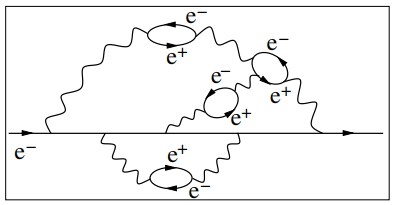
\includegraphics[width=0.5\textwidth,height=0.3\textwidth]{chapter1/img/screening}
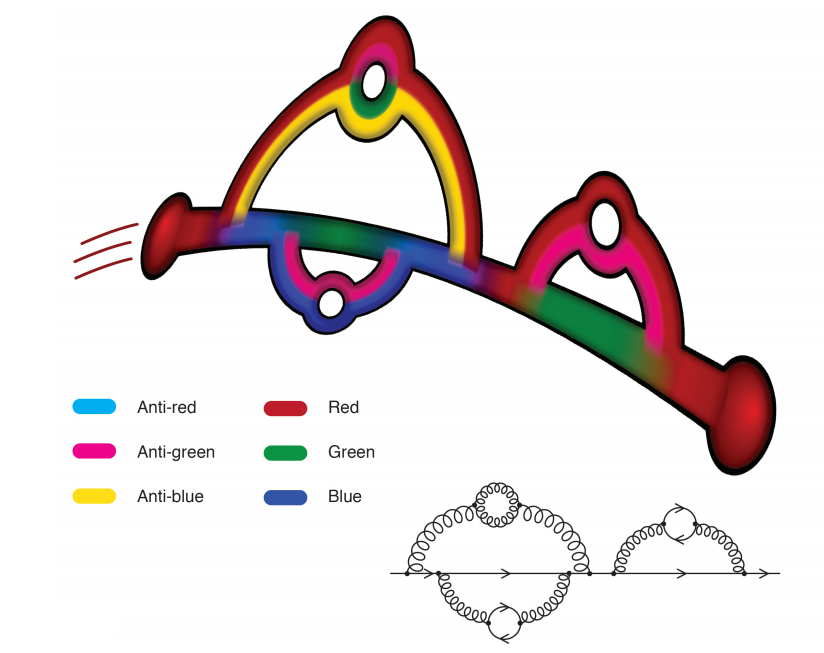
\includegraphics[width=0.5\textwidth,height=0.3\textwidth]{chapter1/img/antiscreening}
\caption{\textit{Left}: virtual pairs of positrons and electrons can be produced in vacuum. Positrons are attracted to the bare electron resulting into an apparent lower charge of the bare particles from larger distances. This effect is referred to as \textit{screening}. \textit{Right}: quark and antiquark pairs have a similar screening effect in color charge as the case for electrical charges. There is an anti-screening effect due to gluons that ``extract'' color from the bare quark and is stronger than the screening effect of quark-antiquark pairs. At small distances, the dilution of the initial color charge is larger than at large distance.  This drawing should not be taken literally and the concept of self-interaction is very hard to illustrate. One could interpret the initial red color with a gluon emission as a conservation of the red color, thus the red quark can only become blue if a gluon with a red and anti-blue color is emitted (gluons need to be color+anti-color pairs). In the first, top loop, two  gluons are created but cannot have a combined color: anti-green with red (first) and green with anti-blue (second) is possible since green and anti-green have a net zero color charge. Figures from \cite{Deur:2016tte}.}
\label{fig:screening}
\end{figure}

\begin{equation}
\beta\left(g\right) = \frac{\partial g}{\partial \log\left(\mu\right)}.
\end{equation}
More coupling in shorter distances (i.e. higher energies) would give rise to a positive beta function and is the case in QED. In QCD, gluons carry a color charge and enter the beta function with a negative sign

\begin{equation}
\beta\left(g\right) = -\left(11 - \frac{2n_f}{3}\right)\frac{g^3}{16\pi^2},
\end{equation}
with $n_f$ the number of fermions that participate in the strong interaction. This decrease in coupling strength in function of energy scale is called \textit{asymptotic freedom}. Alternatively, we can write down the coupling constants in function of the energy 

\begin{equation}
\alpha^{-1}_i \left(Q\right) = \alpha^{-1}_{i}\left(m_Z\right) + \frac{b_i}{2\pi}\log\frac{Q}{m_Z},
\end{equation}
with $b_1 = -\frac{4}{3}n_g - \frac{1}{10}n_h$, $b_2 = \frac{22}{3}-\frac{4}{3}n_g-\frac{1}{6}$ and $b_3 = \frac{11}{-\frac{4}{3}}$ the U(1), SU(2) and
SU(3) constants in which $n_g$ denotes the  number of quark and lepton generations and $n_h$ is the number of Higgs doublet fields. These three couplings seem to converge, leading people to believe a more universal theory at higher energies would unify these parameters into one and is shown in Figure \ref{fig:running}.
\fi
%END LEAVING OUT

\begin{figure}
\centering
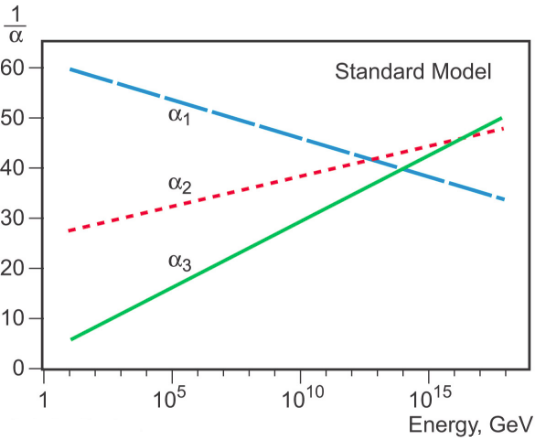
\includegraphics[width = 0.5\textwidth]{chapter1/img/running}
\caption{Running of the coupling constants in the Standard Model. Figure from \cite{nobel2004url}.}
\label{fig:running}
\end{figure}

\subsection{Unifying theories}
\label{sub:unifying}
Linking the seemingly arbitrary parameters in the Standard Model has been ongoing for the last couple of decades. Combining these theories is not straightforward since they exhibit very different behaviors. Electromagnetism is long-ranged, the weak force is short-ranged and the strong force is weak in high-energy environments such as the early universe and strong where the probing energy is low. Many GUTs predict that quarks and leptons are part of a single representation of a gauge group with one single hypercharge and would explain why the electric charge of electrons and protons seem to be exactly the same \cite{He:1989eq}.

The simplest GUT is SU(5), which would break down into the Standard Model at lower energies due to spontaneous symmetry breaking. Other possible extensions are, for example, SO(10) \cite{Bertolini:2009qj}, SU(8) \cite{Yu:1984pb} and O(16) Lie groups. Another example is string theory, a theoretical framework that starts with the idea that point-like particles of particle physics can be replaced by one-dimensional objects called strings. These strings can propagate through space and interact with each other. Properties that we are more familiar with, such as charge, mass, etc. are determined by the vibrational state of the strings.

Unfortunately, the full theory does not have a definition in all circumstances and describes an enormous landscape of possible universes and is mainly used to describe quantum gravity. However, charge quantization is often not assumed in string theory, making particles with an anomalous charge plausible \cite{Wen:1985qj,Athanasiu:1988uj}.\\


\noindent Without experimental results there is still much ongoing debate into which theory is the correct one. There are many more theories aside from the possible extentions that are listed here such as Supersymmetry, Little Higgs, Technicolor... but go beyond the scope of this work.

\iffalse
\subsubsection*{Supersymmetry}
Supersymmetric models impose a new symmetry, supersymmetry (SUSY), that relates fermions and bosons. Every fermion would have a, yet unseen, bosonic supersymmetric partner and vice versa. This theory is highly motivated due to its ability in canceling the quadratically divergent terms in the mass correction of the Higgs boson. More specifically, because the Higgs couples to massive particles there will be a correction to the bare Higgs mass due to these couplings. By applying the Feynman rules, the quantum corrections to the Higgs mass squared from fermions is 

\begin{equation}
\label{eq:higgscorrections}
\Delta m^2_H = -\frac{\left| \lambda_f \right|^2}{8\pi^2} \left[ \Lambda^2_{UV}+...\right],
\end{equation}
\noindent where $\Lambda_{UV}$ is the ultraviolet cutoff. If we assume this to be of the order of the Planck mass, this would lead to extremely small numbers for the Yukawa coupling constants $\lambda_f$.

Alternatively, the corrections from two additional complex scalors with similar couplings to the Higgs ($\lambda_s = \left|\lambda_f\right|^2$) is equal to

\begin{equation}
\Delta m^2_H = 2 \times \frac{\lambda_s}{16\pi^2}\left[ \Lambda^2_{UV}+... \right]
\end{equation}
and are able to cancel the fermion contributions. Unbroken SUSY would lead to partners with the same mass as the particles we know from the SM and would have been discovered long ago. Because of this, one assumes the symmetry to be broken.

The last couple of years, SUSY was regarded as the most promising extension of the SM with tremendous efforts from big collaborations such as the experiments at the Large Hadron Collidor (LHC) in search for proof. Unfortunately, to this date no evidence for SUSY has been found.

\subsubsection*{Little Higgs}
The basic motivation for a Little Higgs scenario comes from the quadratic one-loop corrections such as in Eq. \ref{eq:higgscorrections}. In Little Higgs scenarios, the Higgs field is a pseudo-Nambu-Goldstone boson of a spontaneously broken symmetry. The symmetry is broken by two sets of interactions and each interaction preserves enough symmetry so that no single interaction gives radiative corrections to the Higgs mass. However, two interactions together do generate a Higgs mass, but the Higgs mass squared terms are suppressed by two loops relative to the cutoff. Because these are proportional to the two coupling strengths, while the Standard Model Higgs only requires a single interaction to generate a mass, it has a lower radiative mass corrections compared to the Standard Model Higgs. The biggest difference in Little Higgs scenarios with Supersymmetry is that it has particles of the same spin that cancel the quadratic divergences to the Higgs mass, i.e. a fermion cancels a quadratic divergence from a fermion. For more information, see Refs. \cite{Cheng:2007bu,Reuter:2012sd}.	

\subsubsection*{String theory}

\fi




\subsection{How to look for new physics}
In general, one could say there are two possible ways to look for new physics. Essentially all of the physics in our solar system can be explained with what we know from the Standard Model. Interactions in controlled laboratory environments are currently on the order of $\sim$10 TeV center of mass energy in the experiments at the LHC. This could still be well below the energy levels to produce new, exotic, particles. In the \underline{energy frontier} it is the goal to reach the highest energies possible in order to get as close to the energy requirements where new physics becomes more prominent. As a consequence, more and more cosmic ray experiments have found an interest in searches for physics beyond the Standard Model. This is sometimes called the \textit{cosmic frontier}. This analysis tries to explore this possibility in more detail for the IceCube experiment. Cosmic ray experiments have the disadvantage that they are not fully contained experiments and information is lost as the primary interaction is unknown and important parameters such as energy, direction, type,... of the particle have to be reconstructed with large uncertainties.

The other approach tries to extract information from precision experiments and is therefore reliant on lowering the statistical and systematical uncertainties. In these experiments, the intensity of the beam of particle accelerators is pushed to its highest value and this is therefore referred to as the \underline{intensity frontier}. This strategy tries to generate huge numbers of particles needed to study rare or exotic subatomic processes. Rare processes could give us a lot of information on unknown physics. Some parameters which can be calculated in the SM have a small offset with respect to what is measured in experiments.

The difference between the two methods can be summarized by saying that new physics at higher energies can produce new particles at high-energy collisions that are sought for in the energy frontier. The higher the scale where new physics enters, the more energy is needed in particle collisions. However, parameters from our current theories that not include new physics could also have a small but measurable offset at lower energies (the ones we are able to probe currently), which is what is measured in the intensity frontier. \\


\noindent I'd like to finish this chapter with quotes from Steven Weinberg in an interview with Nova about his vision on string theory. It shows the apparent stalemate physicists seem to find themselves in: there are no theoretical breakthroughs regarding long standing problems.

\begin{center}
\begin{minipage}[5cm]{0.9\textwidth}
\textit{``I believe that there is a simple theory that governs everything—the four forces we know about, perhaps other forces as well. I'm not sure that's true. It may be that nature is irreducibly messy. I'm sure that we should assume it's not, because otherwise we're never going to find a fundamental theory. But even so, we're not guaranteed that we'll find it. We may not be smart enough. Dogs are not smart enough to understand quantum mechanics. I'm not sure that people are smart enough to understand the whatever-it-is that unifies everything. I think we probably are, because of our ability to link our minds through language, but I'm not certain.''}
\end{minipage} 
\end{center}

\begin{center}
\begin{minipage}[5cm]{0.9\textwidth}
\textit{\noindent ``There was a marvelous period from, I'd say, the mid-'60s until the late '70s when theoretical physicists actually had something to say that experimentalists were interested in. Experimentalists made discoveries that theoretical physicists were interested in. Everything was converging toward a simple picture of the known particles and forces, a picture that eventually became known as the Standard Model. I think I gave it that name. And it was a time when graduate students would run through the halls of a physics building saying they had discovered another particle and it fit the theories, and it was all so exciting.''}
\end{minipage} 
\end{center}

\begin{center}
\begin{minipage}[5cm]{0.9\textwidth}
\textit{\noindent ``Since the late '70s, I'd say, particle physics has been in somewhat of a doldrums. Partly it's just the price we're paying for the great success we had in that wonderful time then. I think cosmology now, for example, is much more exciting than particle physics. The string theorists are trying to push ahead without much support from relevant experiments, because there aren't any relevant experiments that can be done at the kind of scales that the string theorists are interested in.''}
\end{minipage} 
\end{center}

\noindent Even though it might take us a long time to find the answers we are looking for, this current stalemate should not prevent us doing more fundamental research. We still do not know everything and it's probably even foolish to think we almost do. Finding some answers might be difficult but probably all the more fulfilling once we have them.